\documentclass[a4paper,twoside,11pt,titlepage]{book}
\usepackage{listings}

\usepackage[utf8]{inputenc}
\usepackage[spanish,es-tabla]{babel}
\usepackage{graphicx}
\usepackage{subcaption}
\usepackage[dvips]{epsfig}
\usepackage{amssymb}
\usepackage{eurosym}
\usepackage{float}
\usepackage{latexsym}
\usepackage{a4}
\usepackage{listings}
\usepackage[hidelinks]{hyperref} 
\usepackage{multirow} % para las tablas
\usepackage{tabularx}

\newcolumntype{C}[1]{>{\centering\arraybackslash}p{#1}} %para determinar ancho de columna centrada
\newcolumntype{L}[1]{>{\arraybackslash}p{#1}} %para determinar ancho de columna de columna a la izquierda

% \usepackage[style=list, number=none]{glossary} %
%\usepackage{titlesec}
%\usepackage{pailatino}

\decimalpoint
\usepackage{dcolumn}
\newcolumntype{.}{D{.}{\esperiod}{-1}}
\makeatletter
\addto\shorthandsspanish{\let\esperiod\es@period@code}
\makeatother


%\usepackage[chapter]{algorithm}
\RequirePackage{verbatim}
%\RequirePackage[Glenn]{fncychap}
\usepackage{fancyhdr}
\usepackage{graphicx}
\usepackage{afterpage}

\usepackage{longtable}

% ********************************************************************
% Re-usable information
% ********************************************************************
\newcommand{\myTitle}{Gestión de juegos conversacionales\xspace}
\newcommand{\myDegree}{Grado en Ingeniería Informática\xspace}
\newcommand{\myName}{Guillermo Muriel Sánchez lafuente\xspace}
\newcommand{\myProf}{Juan Julián Merelo Guervós\xspace}
\newcommand{\myOtherProf}{Nombre Apllido1 Apellido2 (tutor2)\xspace}
%\newcommand{\mySupervisor}{Put name here\xspace}
\newcommand{\myFaculty}{Escuela Técnica Superior de Ingenierías Informática y de
Telecomunicación\xspace}
\newcommand{\myFacultyShort}{E.T.S. de Ingenierías Informática y de
Telecomunicación\xspace}
\newcommand{\myDepartment}{Departamento de Arquitectura y Tecnología de Computadores\xspace}
\newcommand{\myUni}{\protect{Universidad de Granada}\xspace}
\newcommand{\myLocation}{Granada\xspace}
\newcommand{\myTime}{\today\xspace}
\newcommand{\myVersion}{Version 1\xspace}


\hypersetup{
pdfauthor = {  \myName (email (en) ugr (punto) es)},
pdftitle = {\myTitle},
pdfsubject = {},
pdfkeywords = {palabra_clave1, palabra_clave2, palabra_clave3, ...},
pdfcreator = {LaTeX con el paquete ....},
pdfproducer = {pdflatex}
}

%\hyphenation{}


%\usepackage{doxygen/doxygen}
%\usepackage{pdfpages}
\usepackage{url}
\usepackage{colortbl,longtable}
\usepackage[stable]{footmisc}
%\usepackage{index}

%\makeindex
%\usepackage[style=long, cols=2,border=plain,toc=true,number=none]{glossary}
% \makeglossary

% Definición de comandos que me son tiles:
%\renewcommand{\indexname}{Índice alfabético}
%\renewcommand{\glossaryname}{Glosario}

\pagestyle{fancy}
\fancyhf{}
\fancyhead[LO]{\leftmark}
\fancyhead[RE]{\rightmark}
\fancyhead[RO,LE]{\textbf{\thepage}}
\renewcommand{\chaptermark}[1]{\markboth{\textbf{#1}}{}}
\renewcommand{\sectionmark}[1]{\markright{\textbf{\thesection. #1}}}

\setlength{\headheight}{1.5\headheight}

\newcommand{\HRule}{\rule{\linewidth}{0.5mm}}
%Definimos los tipos teorema, ejemplo y definición podremos usar estos tipos
%simplemente poniendo \begin{teorema} \end{teorema} ...
\newtheorem{teorema}{Teorema}[chapter]
\newtheorem{ejemplo}{Ejemplo}[chapter]
\newtheorem{definicion}{Definición}[chapter]

\definecolor{gray97}{gray}{.97}
\definecolor{gray75}{gray}{.75}
\definecolor{gray45}{gray}{.45}
\definecolor{gray30}{gray}{.94}

\lstset{ frame=Ltb,
     framerule=0.5pt,
     aboveskip=0.5cm,
     framextopmargin=3pt,
     framexbottommargin=3pt,
     framexleftmargin=0.1cm,
     framesep=0pt,
     rulesep=.4pt,
     backgroundcolor=\color{gray97},
     rulesepcolor=\color{black},
     %
     stringstyle=\ttfamily,
     showstringspaces = false,
     basicstyle=\scriptsize\ttfamily,
     commentstyle=\color{gray45},
     keywordstyle=\bfseries,
     %
     numbers=left,
     numbersep=6pt,
     numberstyle=\tiny,
     numberfirstline = false,
     breaklines=true,
   }
 
% minimizar fragmentado de listados
\lstnewenvironment{listing}[1][]
   {\lstset{#1}\pagebreak[0]}{\pagebreak[0]}

\lstdefinestyle{CodigoC}
   {
	basicstyle=\scriptsize,
	frame=single,
	language=C,
	numbers=left
   }
\lstdefinestyle{CodigoC++}
   {
	basicstyle=\small,
	frame=single,
	backgroundcolor=\color{gray30},
	language=C++,
	numbers=left
   }

 
\lstdefinestyle{Consola}
   {basicstyle=\scriptsize\bf\ttfamily,
    backgroundcolor=\color{gray30},
    frame=single,
    numbers=none
   }


\newcommand{\bigrule}{\titlerule[0.5mm]}


%Para conseguir que en las páginas en blanco no ponga cabecerass
\makeatletter
\def\clearpage{%
  \ifvmode
    \ifnum \@dbltopnum =\m@ne
      \ifdim \pagetotal <\topskip
        \hbox{}
      \fi
    \fi
  \fi
  \newpage
  \thispagestyle{empty}
  \write\m@ne{}
  \vbox{}
  \penalty -\@Mi
}
\makeatother

\usepackage{pdfpages}

\begin{document}
\begin{titlepage}
 
 
\newlength{\centeroffset}
\setlength{\centeroffset}{-0.5\oddsidemargin}
\addtolength{\centeroffset}{0.5\evensidemargin}
\thispagestyle{empty}

\noindent\hspace*{\centeroffset}\begin{minipage}{\textwidth}

\centering

\includegraphics[width=0.9\textwidth]{imagenes/logo_ugr.jpg}\\[1.4cm]

\textsc{ \Large TRABAJO FIN DE GRADO\\[0.2cm]}
\textsc{ INGENIERÍA EN ...}\\[1cm]
% Upper part of the page
% 
% Title
{\Huge\bfseries Titulo del Proyecto\\
}
\noindent\rule[-1ex]{\textwidth}{3pt}\\[3.5ex]
{\large\bfseries Subtitulo del Proyecto}
\end{minipage}

\vspace{2.5cm}
\noindent\hspace*{\centeroffset}\begin{minipage}{\textwidth}
\centering

\textbf{Autor}\\ {\myName}\\[2.5ex]
\textbf{Directores}\\
{Nombre Apellido1 Apellido2 (tutor1)\\
Nombre Apellido1 Apellido2 (tutor2)}\\[2cm]

\includegraphics[width=0.3\textwidth]{imagenes/etsiit_logo.png}\\[0.1cm]
\textsc{Escuela Técnica Superior de Ingenierías Informática y de Telecomunicación}\\
\textsc{---}\\
Granada, mes de 201
\end{minipage}
%\addtolength{\textwidth}{\centeroffset}
%\vspace{\stretch{2}}
\end{titlepage}



\chapter*{}
%\thispagestyle{empty}
%\cleardoublepage

%\thispagestyle{empty}

\begin{titlepage}
 
 
\setlength{\centeroffset}{-0.5\oddsidemargin}
\addtolength{\centeroffset}{0.5\evensidemargin}
\thispagestyle{empty}

\noindent\hspace*{\centeroffset}\begin{minipage}{\textwidth}

\centering
%
\includegraphics[width=0.9\textwidth]{imagenes/logo_ugr.jpg}\\[1.4cm]

%\textsc{ \Large PROYECTO FIN DE CARRERA\\[0.2cm]}
%\textsc{ INGENIERÍA EN INFORMÁTICA}\\[1cm]
% Upper part of the page
% 

 \vspace{3.3cm}

%si el proyecto tiene logo poner aquí

\includegraphics{imagenes/logo_riddling.png} 
 \vspace{0.5cm}

% Title

{\Huge\bfseries \myTitle\\
}
\noindent\rule[-1ex]{\textwidth}{3pt}\\[3.5ex]
{\large\bfseries Una aplicación en la nube\\[4cm]}
\end{minipage}

\vspace{2.5cm}
\noindent\hspace*{\centeroffset}\begin{minipage}{\textwidth}
\centering

\textbf{Autor}\\ \myName\\[2.5ex]
\textbf{Directores}\\\myProf\\[2cm]
%
\includegraphics[width=0.15\textwidth]{imagenes/tstc.png}\\[0.1cm]
\textsc\myDepartment\\
%\textsc{---}\\
Granada, septiembre de 2018
\end{minipage}
%\addtolength{\textwidth}{\centeroffset}
\vspace{\stretch{2}}

 
\end{titlepage}






\cleardoublepage
\thispagestyle{empty}

\begin{center}
{\large\bfseries Título del Proyecto: Subtítulo del proyecto}\\
\end{center}
\begin{center}
Nombre Apellido1 Apellido2 (alumno)\\
\end{center}

%\vspace{0.7cm}
\noindent{\textbf{Palabras clave}: palabra\_clave1, palabra\_clave2, palabra\_clave3, ......}\\

\vspace{0.7cm}
\noindent{\textbf{Resumen}}\\

Poner aquí el resumen.
\cleardoublepage


\thispagestyle{empty}


\begin{center}
{\large\bfseries Project Title: Project Subtitle}\\
\end{center}
\begin{center}
First name, Family name (student)\\
\end{center}

%\vspace{0.7cm}
\noindent{\textbf{Keywords}: Keyword1, Keyword2, Keyword3, ....}\\

\vspace{0.7cm}
\noindent{\textbf{Abstract}}\\

Write here the abstract in English.

\chapter*{}
\thispagestyle{empty}

\noindent\rule[-1ex]{\textwidth}{2pt}\\[4.5ex]

Yo, \textbf{Nombre Apellido1 Apellido2}, alumno de la titulación TITULACIÓN de la \textbf{Escuela Técnica Superior
de Ingenierías Informática y de Telecomunicación de la Universidad de Granada}, con DNI XXXXXXXXX, autorizo la
ubicación de la siguiente copia de mi Trabajo Fin de Grado en la biblioteca del centro para que pueda ser
consultada por las personas que lo deseen.

\vspace{6cm}

\noindent Fdo: Nombre Apellido1 Apellido2

\vspace{2cm}

\begin{flushright}
Granada a X de mes de 201 .
\end{flushright}


\chapter*{}
\thispagestyle{empty}

\noindent\rule[-1ex]{\textwidth}{2pt}\\[4.5ex]

D. \textbf{Nombre Apellido1 Apellido2 (tutor1)}, Profesor del Área de XXXX del Departamento YYYY de la Universidad de Granada.

\vspace{0.5cm}

D. \textbf{Nombre Apellido1 Apellido2 (tutor2)}, Profesor del Área de XXXX del Departamento YYYY de la Universidad de Granada.


\vspace{0.5cm}

\textbf{Informan:}

\vspace{0.5cm}

Que el presente trabajo, titulado \textit{\textbf{Título del proyecto, Subtítulo del proyecto}},
ha sido realizado bajo su supervisión por \textbf{Nombre Apellido1 Apellido2 (alumno)}, y autorizamos la defensa de dicho trabajo ante el tribunal
que corresponda.

\vspace{0.5cm}

Y para que conste, expiden y firman el presente informe en Granada a X de mes de 201 .

\vspace{1cm}

\textbf{Los directores:}

\vspace{5cm}

\noindent \textbf{Nombre Apellido1 Apellido2 (tutor1) \ \ \ \ \ Nombre Apellido1 Apellido2 (tutor2)}

\chapter*{Agradecimientos}
\thispagestyle{empty}

       \vspace{1cm}


Poner aquí agradecimientos...



\chapter*{}
\title{GNU GENERAL PUBLIC LICENSE}
\date{Version 3, 29 June 2007}

\maketitle

\begin{center}
{\parindent 0in

Copyright \copyright\  2007 Free Software Foundation, Inc. \texttt{https://fsf.org/}

\bigskip
Everyone is permitted to copy and distribute verbatim copies of this

license document, but changing it is not allowed.}

\end{center}

\renewcommand{\abstractname}{Preamble}
\begin{abstract}
The GNU General Public License is a free, copyleft license for
software and other kinds of works.

The licenses for most software and other practical works are designed
to take away your freedom to share and change the works.  By contrast,
the GNU General Public License is intended to guarantee your freedom to
share and change all versions of a program--to make sure it remains free
software for all its users.  We, the Free Software Foundation, use the
GNU General Public License for most of our software; it applies also to
any other work released this way by its authors.  You can apply it to
your programs, too.

When we speak of free software, we are referring to freedom, not
price.  Our General Public Licenses are designed to make sure that you
have the freedom to distribute copies of free software (and charge for
them if you wish), that you receive source code or can get it if you
want it, that you can change the software or use pieces of it in new
free programs, and that you know you can do these things.

To protect your rights, we need to prevent others from denying you
these rights or asking you to surrender the rights.  Therefore, you have
certain responsibilities if you distribute copies of the software, or if
you modify it: responsibilities to respect the freedom of others.

For example, if you distribute copies of such a program, whether
gratis or for a fee, you must pass on to the recipients the same
freedoms that you received.  You must make sure that they, too, receive
or can get the source code.  And you must show them these terms so they
know their rights.

Developers that use the GNU GPL protect your rights with two steps:
(1) assert copyright on the software, and (2) offer you this License
giving you legal permission to copy, distribute and/or modify it.

For the developers' and authors' protection, the GPL clearly explains
that there is no warranty for this free software.  For both users' and
authors' sake, the GPL requires that modified versions be marked as
changed, so that their problems will not be attributed erroneously to
authors of previous versions.

Some devices are designed to deny users access to install or run
modified versions of the software inside them, although the manufacturer
can do so.  This is fundamentally incompatible with the aim of
protecting users' freedom to change the software.  The systematic
pattern of such abuse occurs in the area of products for individuals to
use, which is precisely where it is most unacceptable.  Therefore, we
have designed this version of the GPL to prohibit the practice for those
products.  If such problems arise substantially in other domains, we
stand ready to extend this provision to those domains in future versions
of the GPL, as needed to protect the freedom of users.

Finally, every program is threatened constantly by software patents.
States should not allow patents to restrict development and use of
software on general-purpose computers, but in those that do, we wish to
avoid the special danger that patents applied to a free program could
make it effectively proprietary.  To prevent this, the GPL assures that
patents cannot be used to render the program non-free.

The precise terms and conditions for copying, distribution and
modification follow.
\end{abstract}

\begin{center}
{\Large \sc Terms and Conditions}
\end{center}


\begin{enumerate}

\addtocounter{enumi}{-1}

\item Definitions.

``This License'' refers to version 3 of the GNU General Public License.

``Copyright'' also means copyright-like laws that apply to other kinds of
works, such as semiconductor masks.

``The Program'' refers to any copyrightable work licensed under this
License.  Each licensee is addressed as ``you''.  ``Licensees'' and
``recipients'' may be individuals or organizations.

To ``modify'' a work means to copy from or adapt all or part of the work
in a fashion requiring copyright permission, other than the making of an
exact copy.  The resulting work is called a ``modified version'' of the
earlier work or a work ``based on'' the earlier work.

A ``covered work'' means either the unmodified Program or a work based
on the Program.

To ``propagate'' a work means to do anything with it that, without
permission, would make you directly or secondarily liable for
infringement under applicable copyright law, except executing it on a
computer or modifying a private copy.  Propagation includes copying,
distribution (with or without modification), making available to the
public, and in some countries other activities as well.

To ``convey'' a work means any kind of propagation that enables other
parties to make or receive copies.  Mere interaction with a user through
a computer network, with no transfer of a copy, is not conveying.

An interactive user interface displays ``Appropriate Legal Notices''
to the extent that it includes a convenient and prominently visible
feature that (1) displays an appropriate copyright notice, and (2)
tells the user that there is no warranty for the work (except to the
extent that warranties are provided), that licensees may convey the
work under this License, and how to view a copy of this License.  If
the interface presents a list of user commands or options, such as a
menu, a prominent item in the list meets this criterion.

\item Source Code.

The ``source code'' for a work means the preferred form of the work
for making modifications to it.  ``Object code'' means any non-source
form of a work.

A ``Standard Interface'' means an interface that either is an official
standard defined by a recognized standards body, or, in the case of
interfaces specified for a particular programming language, one that
is widely used among developers working in that language.

The ``System Libraries'' of an executable work include anything, other
than the work as a whole, that (a) is included in the normal form of
packaging a Major Component, but which is not part of that Major
Component, and (b) serves only to enable use of the work with that
Major Component, or to implement a Standard Interface for which an
implementation is available to the public in source code form.  A
``Major Component'', in this context, means a major essential component
(kernel, window system, and so on) of the specific operating system
(if any) on which the executable work runs, or a compiler used to
produce the work, or an object code interpreter used to run it.

The ``Corresponding Source'' for a work in object code form means all
the source code needed to generate, install, and (for an executable
work) run the object code and to modify the work, including scripts to
control those activities.  However, it does not include the work's
System Libraries, or general-purpose tools or generally available free
programs which are used unmodified in performing those activities but
which are not part of the work.  For example, Corresponding Source
includes interface definition files associated with source files for
the work, and the source code for shared libraries and dynamically
linked subprograms that the work is specifically designed to require,
such as by intimate data communication or control flow between those
subprograms and other parts of the work.

The Corresponding Source need not include anything that users
can regenerate automatically from other parts of the Corresponding
Source.

The Corresponding Source for a work in source code form is that
same work.

\item Basic Permissions.

All rights granted under this License are granted for the term of
copyright on the Program, and are irrevocable provided the stated
conditions are met.  This License explicitly affirms your unlimited
permission to run the unmodified Program.  The output from running a
covered work is covered by this License only if the output, given its
content, constitutes a covered work.  This License acknowledges your
rights of fair use or other equivalent, as provided by copyright law.

You may make, run and propagate covered works that you do not
convey, without conditions so long as your license otherwise remains
in force.  You may convey covered works to others for the sole purpose
of having them make modifications exclusively for you, or provide you
with facilities for running those works, provided that you comply with
the terms of this License in conveying all material for which you do
not control copyright.  Those thus making or running the covered works
for you must do so exclusively on your behalf, under your direction
and control, on terms that prohibit them from making any copies of
your copyrighted material outside their relationship with you.

Conveying under any other circumstances is permitted solely under
the conditions stated below.  Sublicensing is not allowed; section 10
makes it unnecessary.

\item Protecting Users' Legal Rights From Anti-Circumvention Law.

No covered work shall be deemed part of an effective technological
measure under any applicable law fulfilling obligations under article
11 of the WIPO copyright treaty adopted on 20 December 1996, or
similar laws prohibiting or restricting circumvention of such
measures.

When you convey a covered work, you waive any legal power to forbid
circumvention of technological measures to the extent such circumvention
is effected by exercising rights under this License with respect to
the covered work, and you disclaim any intention to limit operation or
modification of the work as a means of enforcing, against the work's
users, your or third parties' legal rights to forbid circumvention of
technological measures.

\item Conveying Verbatim Copies.

You may convey verbatim copies of the Program's source code as you
receive it, in any medium, provided that you conspicuously and
appropriately publish on each copy an appropriate copyright notice;
keep intact all notices stating that this License and any
non-permissive terms added in accord with section 7 apply to the code;
keep intact all notices of the absence of any warranty; and give all
recipients a copy of this License along with the Program.

You may charge any price or no price for each copy that you convey,
and you may offer support or warranty protection for a fee.

\item Conveying Modified Source Versions.

You may convey a work based on the Program, or the modifications to
produce it from the Program, in the form of source code under the
terms of section 4, provided that you also meet all of these conditions:
  \begin{enumerate}
  \item The work must carry prominent notices stating that you modified
  it, and giving a relevant date.

  \item The work must carry prominent notices stating that it is
  released under this License and any conditions added under section
  7.  This requirement modifies the requirement in section 4 to
  ``keep intact all notices''.

  \item You must license the entire work, as a whole, under this
  License to anyone who comes into possession of a copy.  This
  License will therefore apply, along with any applicable section 7
  additional terms, to the whole of the work, and all its parts,
  regardless of how they are packaged.  This License gives no
  permission to license the work in any other way, but it does not
  invalidate such permission if you have separately received it.

  \item If the work has interactive user interfaces, each must display
  Appropriate Legal Notices; however, if the Program has interactive
  interfaces that do not display Appropriate Legal Notices, your
  work need not make them do so.
\end{enumerate}
A compilation of a covered work with other separate and independent
works, which are not by their nature extensions of the covered work,
and which are not combined with it such as to form a larger program,
in or on a volume of a storage or distribution medium, is called an
``aggregate'' if the compilation and its resulting copyright are not
used to limit the access or legal rights of the compilation's users
beyond what the individual works permit.  Inclusion of a covered work
in an aggregate does not cause this License to apply to the other
parts of the aggregate.

\item Conveying Non-Source Forms.

You may convey a covered work in object code form under the terms
of sections 4 and 5, provided that you also convey the
machine-readable Corresponding Source under the terms of this License,
in one of these ways:
  \begin{enumerate}
  \item Convey the object code in, or embodied in, a physical product
  (including a physical distribution medium), accompanied by the
  Corresponding Source fixed on a durable physical medium
  customarily used for software interchange.

  \item Convey the object code in, or embodied in, a physical product
  (including a physical distribution medium), accompanied by a
  written offer, valid for at least three years and valid for as
  long as you offer spare parts or customer support for that product
  model, to give anyone who possesses the object code either (1) a
  copy of the Corresponding Source for all the software in the
  product that is covered by this License, on a durable physical
  medium customarily used for software interchange, for a price no
  more than your reasonable cost of physically performing this
  conveying of source, or (2) access to copy the
  Corresponding Source from a network server at no charge.

  \item Convey individual copies of the object code with a copy of the
  written offer to provide the Corresponding Source.  This
  alternative is allowed only occasionally and noncommercially, and
  only if you received the object code with such an offer, in accord
  with subsection 6b.

  \item Convey the object code by offering access from a designated
  place (gratis or for a charge), and offer equivalent access to the
  Corresponding Source in the same way through the same place at no
  further charge.  You need not require recipients to copy the
  Corresponding Source along with the object code.  If the place to
  copy the object code is a network server, the Corresponding Source
  may be on a different server (operated by you or a third party)
  that supports equivalent copying facilities, provided you maintain
  clear directions next to the object code saying where to find the
  Corresponding Source.  Regardless of what server hosts the
  Corresponding Source, you remain obligated to ensure that it is
  available for as long as needed to satisfy these requirements.

  \item Convey the object code using peer-to-peer transmission, provided
  you inform other peers where the object code and Corresponding
  Source of the work are being offered to the general public at no
  charge under subsection 6d.
  \end{enumerate}

A separable portion of the object code, whose source code is excluded
from the Corresponding Source as a System Library, need not be
included in conveying the object code work.

A ``User Product'' is either (1) a ``consumer product'', which means any
tangible personal property which is normally used for personal, family,
or household purposes, or (2) anything designed or sold for incorporation
into a dwelling.  In determining whether a product is a consumer product,
doubtful cases shall be resolved in favor of coverage.  For a particular
product received by a particular user, ``normally used'' refers to a
typical or common use of that class of product, regardless of the status
of the particular user or of the way in which the particular user
actually uses, or expects or is expected to use, the product.  A product
is a consumer product regardless of whether the product has substantial
commercial, industrial or non-consumer uses, unless such uses represent
the only significant mode of use of the product.

``Installation Information'' for a User Product means any methods,
procedures, authorization keys, or other information required to install
and execute modified versions of a covered work in that User Product from
a modified version of its Corresponding Source.  The information must
suffice to ensure that the continued functioning of the modified object
code is in no case prevented or interfered with solely because
modification has been made.

If you convey an object code work under this section in, or with, or
specifically for use in, a User Product, and the conveying occurs as
part of a transaction in which the right of possession and use of the
User Product is transferred to the recipient in perpetuity or for a
fixed term (regardless of how the transaction is characterized), the
Corresponding Source conveyed under this section must be accompanied
by the Installation Information.  But this requirement does not apply
if neither you nor any third party retains the ability to install
modified object code on the User Product (for example, the work has
been installed in ROM).

The requirement to provide Installation Information does not include a
requirement to continue to provide support service, warranty, or updates
for a work that has been modified or installed by the recipient, or for
the User Product in which it has been modified or installed.  Access to a
network may be denied when the modification itself materially and
adversely affects the operation of the network or violates the rules and
protocols for communication across the network.

Corresponding Source conveyed, and Installation Information provided,
in accord with this section must be in a format that is publicly
documented (and with an implementation available to the public in
source code form), and must require no special password or key for
unpacking, reading or copying.

\item Additional Terms.

``Additional permissions'' are terms that supplement the terms of this
License by making exceptions from one or more of its conditions.
Additional permissions that are applicable to the entire Program shall
be treated as though they were included in this License, to the extent
that they are valid under applicable law.  If additional permissions
apply only to part of the Program, that part may be used separately
under those permissions, but the entire Program remains governed by
this License without regard to the additional permissions.

When you convey a copy of a covered work, you may at your option
remove any additional permissions from that copy, or from any part of
it.  (Additional permissions may be written to require their own
removal in certain cases when you modify the work.)  You may place
additional permissions on material, added by you to a covered work,
for which you have or can give appropriate copyright permission.

Notwithstanding any other provision of this License, for material you
add to a covered work, you may (if authorized by the copyright holders of
that material) supplement the terms of this License with terms:
  \begin{enumerate}
  \item Disclaiming warranty or limiting liability differently from the
  terms of sections 15 and 16 of this License; or

  \item Requiring preservation of specified reasonable legal notices or
  author attributions in that material or in the Appropriate Legal
  Notices displayed by works containing it; or

  \item Prohibiting misrepresentation of the origin of that material, or
  requiring that modified versions of such material be marked in
  reasonable ways as different from the original version; or

  \item Limiting the use for publicity purposes of names of licensors or
  authors of the material; or

  \item Declining to grant rights under trademark law for use of some
  trade names, trademarks, or service marks; or

  \item Requiring indemnification of licensors and authors of that
  material by anyone who conveys the material (or modified versions of
  it) with contractual assumptions of liability to the recipient, for
  any liability that these contractual assumptions directly impose on
  those licensors and authors.
  \end{enumerate}

All other non-permissive additional terms are considered ``further
restrictions'' within the meaning of section 10.  If the Program as you
received it, or any part of it, contains a notice stating that it is
governed by this License along with a term that is a further
restriction, you may remove that term.  If a license document contains
a further restriction but permits relicensing or conveying under this
License, you may add to a covered work material governed by the terms
of that license document, provided that the further restriction does
not survive such relicensing or conveying.

If you add terms to a covered work in accord with this section, you
must place, in the relevant source files, a statement of the
additional terms that apply to those files, or a notice indicating
where to find the applicable terms.

Additional terms, permissive or non-permissive, may be stated in the
form of a separately written license, or stated as exceptions;
the above requirements apply either way.

\item Termination.

You may not propagate or modify a covered work except as expressly
provided under this License.  Any attempt otherwise to propagate or
modify it is void, and will automatically terminate your rights under
this License (including any patent licenses granted under the third
paragraph of section 11).

However, if you cease all violation of this License, then your
license from a particular copyright holder is reinstated (a)
provisionally, unless and until the copyright holder explicitly and
finally terminates your license, and (b) permanently, if the copyright
holder fails to notify you of the violation by some reasonable means
prior to 60 days after the cessation.

Moreover, your license from a particular copyright holder is
reinstated permanently if the copyright holder notifies you of the
violation by some reasonable means, this is the first time you have
received notice of violation of this License (for any work) from that
copyright holder, and you cure the violation prior to 30 days after
your receipt of the notice.

Termination of your rights under this section does not terminate the
licenses of parties who have received copies or rights from you under
this License.  If your rights have been terminated and not permanently
reinstated, you do not qualify to receive new licenses for the same
material under section 10.

\item Acceptance Not Required for Having Copies.

You are not required to accept this License in order to receive or
run a copy of the Program.  Ancillary propagation of a covered work
occurring solely as a consequence of using peer-to-peer transmission
to receive a copy likewise does not require acceptance.  However,
nothing other than this License grants you permission to propagate or
modify any covered work.  These actions infringe copyright if you do
not accept this License.  Therefore, by modifying or propagating a
covered work, you indicate your acceptance of this License to do so.

\item Automatic Licensing of Downstream Recipients.

Each time you convey a covered work, the recipient automatically
receives a license from the original licensors, to run, modify and
propagate that work, subject to this License.  You are not responsible
for enforcing compliance by third parties with this License.

An ``entity transaction'' is a transaction transferring control of an
organization, or substantially all assets of one, or subdividing an
organization, or merging organizations.  If propagation of a covered
work results from an entity transaction, each party to that
transaction who receives a copy of the work also receives whatever
licenses to the work the party's predecessor in interest had or could
give under the previous paragraph, plus a right to possession of the
Corresponding Source of the work from the predecessor in interest, if
the predecessor has it or can get it with reasonable efforts.

You may not impose any further restrictions on the exercise of the
rights granted or affirmed under this License.  For example, you may
not impose a license fee, royalty, or other charge for exercise of
rights granted under this License, and you may not initiate litigation
(including a cross-claim or counterclaim in a lawsuit) alleging that
any patent claim is infringed by making, using, selling, offering for
sale, or importing the Program or any portion of it.

\item Patents.

A ``contributor'' is a copyright holder who authorizes use under this
License of the Program or a work on which the Program is based.  The
work thus licensed is called the contributor's ``contributor version''.

A contributor's ``essential patent claims'' are all patent claims
owned or controlled by the contributor, whether already acquired or
hereafter acquired, that would be infringed by some manner, permitted
by this License, of making, using, or selling its contributor version,
but do not include claims that would be infringed only as a
consequence of further modification of the contributor version.  For
purposes of this definition, ``control'' includes the right to grant
patent sublicenses in a manner consistent with the requirements of
this License.

Each contributor grants you a non-exclusive, worldwide, royalty-free
patent license under the contributor's essential patent claims, to
make, use, sell, offer for sale, import and otherwise run, modify and
propagate the contents of its contributor version.

In the following three paragraphs, a ``patent license'' is any express
agreement or commitment, however denominated, not to enforce a patent
(such as an express permission to practice a patent or covenant not to
sue for patent infringement).  To ``grant'' such a patent license to a
party means to make such an agreement or commitment not to enforce a
patent against the party.

If you convey a covered work, knowingly relying on a patent license,
and the Corresponding Source of the work is not available for anyone
to copy, free of charge and under the terms of this License, through a
publicly available network server or other readily accessible means,
then you must either (1) cause the Corresponding Source to be so
available, or (2) arrange to deprive yourself of the benefit of the
patent license for this particular work, or (3) arrange, in a manner
consistent with the requirements of this License, to extend the patent
license to downstream recipients.  ``Knowingly relying'' means you have
actual knowledge that, but for the patent license, your conveying the
covered work in a country, or your recipient's use of the covered work
in a country, would infringe one or more identifiable patents in that
country that you have reason to believe are valid.

If, pursuant to or in connection with a single transaction or
arrangement, you convey, or propagate by procuring conveyance of, a
covered work, and grant a patent license to some of the parties
receiving the covered work authorizing them to use, propagate, modify
or convey a specific copy of the covered work, then the patent license
you grant is automatically extended to all recipients of the covered
work and works based on it.

A patent license is ``discriminatory'' if it does not include within
the scope of its coverage, prohibits the exercise of, or is
conditioned on the non-exercise of one or more of the rights that are
specifically granted under this License.  You may not convey a covered
work if you are a party to an arrangement with a third party that is
in the business of distributing software, under which you make payment
to the third party based on the extent of your activity of conveying
the work, and under which the third party grants, to any of the
parties who would receive the covered work from you, a discriminatory
patent license (a) in connection with copies of the covered work
conveyed by you (or copies made from those copies), or (b) primarily
for and in connection with specific products or compilations that
contain the covered work, unless you entered into that arrangement,
or that patent license was granted, prior to 28 March 2007.

Nothing in this License shall be construed as excluding or limiting
any implied license or other defenses to infringement that may
otherwise be available to you under applicable patent law.

\item No Surrender of Others' Freedom.

If conditions are imposed on you (whether by court order, agreement or
otherwise) that contradict the conditions of this License, they do not
excuse you from the conditions of this License.  If you cannot convey a
covered work so as to satisfy simultaneously your obligations under this
License and any other pertinent obligations, then as a consequence you may
not convey it at all.  For example, if you agree to terms that obligate you
to collect a royalty for further conveying from those to whom you convey
the Program, the only way you could satisfy both those terms and this
License would be to refrain entirely from conveying the Program.

\item Use with the GNU Affero General Public License.

Notwithstanding any other provision of this License, you have
permission to link or combine any covered work with a work licensed
under version 3 of the GNU Affero General Public License into a single
combined work, and to convey the resulting work.  The terms of this
License will continue to apply to the part which is the covered work,
but the special requirements of the GNU Affero General Public License,
section 13, concerning interaction through a network will apply to the
combination as such.

\item Revised Versions of this License.

The Free Software Foundation may publish revised and/or new versions of
the GNU General Public License from time to time.  Such new versions will
be similar in spirit to the present version, but may differ in detail to
address new problems or concerns.

Each version is given a distinguishing version number.  If the
Program specifies that a certain numbered version of the GNU General
Public License ``or any later version'' applies to it, you have the
option of following the terms and conditions either of that numbered
version or of any later version published by the Free Software
Foundation.  If the Program does not specify a version number of the
GNU General Public License, you may choose any version ever published
by the Free Software Foundation.

If the Program specifies that a proxy can decide which future
versions of the GNU General Public License can be used, that proxy's
public statement of acceptance of a version permanently authorizes you
to choose that version for the Program.

Later license versions may give you additional or different
permissions.  However, no additional obligations are imposed on any
author or copyright holder as a result of your choosing to follow a
later version.

\item Disclaimer of Warranty.

\begin{sloppypar}
 THERE IS NO WARRANTY FOR THE PROGRAM, TO THE EXTENT PERMITTED BY
 APPLICABLE LAW.  EXCEPT WHEN OTHERWISE STATED IN WRITING THE
 COPYRIGHT HOLDERS AND/OR OTHER PARTIES PROVIDE THE PROGRAM ``AS IS''
 WITHOUT WARRANTY OF ANY KIND, EITHER EXPRESSED OR IMPLIED,
 INCLUDING, BUT NOT LIMITED TO, THE IMPLIED WARRANTIES OF
 MERCHANTABILITY AND FITNESS FOR A PARTICULAR PURPOSE.  THE ENTIRE
 RISK AS TO THE QUALITY AND PERFORMANCE OF THE PROGRAM IS WITH YOU.
 SHOULD THE PROGRAM PROVE DEFECTIVE, YOU ASSUME THE COST OF ALL
 NECESSARY SERVICING, REPAIR OR CORRECTION.
\end{sloppypar}

\item Limitation of Liability.

 IN NO EVENT UNLESS REQUIRED BY APPLICABLE LAW OR AGREED TO IN
 WRITING WILL ANY COPYRIGHT HOLDER, OR ANY OTHER PARTY WHO MODIFIES
 AND/OR CONVEYS THE PROGRAM AS PERMITTED ABOVE, BE LIABLE TO YOU FOR
 DAMAGES, INCLUDING ANY GENERAL, SPECIAL, INCIDENTAL OR CONSEQUENTIAL
 DAMAGES ARISING OUT OF THE USE OR INABILITY TO USE THE PROGRAM
 (INCLUDING BUT NOT LIMITED TO LOSS OF DATA OR DATA BEING RENDERED
 INACCURATE OR LOSSES SUSTAINED BY YOU OR THIRD PARTIES OR A FAILURE
 OF THE PROGRAM TO OPERATE WITH ANY OTHER PROGRAMS), EVEN IF SUCH
 HOLDER OR OTHER PARTY HAS BEEN ADVISED OF THE POSSIBILITY OF SUCH
 DAMAGES.

\item Interpretation of Sections 15 and 16.

If the disclaimer of warranty and limitation of liability provided
above cannot be given local legal effect according to their terms,
reviewing courts shall apply local law that most closely approximates
an absolute waiver of all civil liability in connection with the
Program, unless a warranty or assumption of liability accompanies a
copy of the Program in return for a fee.

\begin{center}
{\Large\sc End of Terms and Conditions}

\bigskip
How to Apply These Terms to Your New Programs
\end{center}

If you develop a new program, and you want it to be of the greatest
possible use to the public, the best way to achieve this is to make it
free software which everyone can redistribute and change under these terms.

To do so, attach the following notices to the program.  It is safest
to attach them to the start of each source file to most effectively
state the exclusion of warranty; and each file should have at least
the ``copyright'' line and a pointer to where the full notice is found.

{\footnotesize
\begin{verbatim}
<one line to give the program's name and a brief idea of what it does.>

Copyright (C) <textyear>  <name of author>

This program is free software: you can redistribute it and/or modify
it under the terms of the GNU General Public License as published by
the Free Software Foundation, either version 3 of the License, or
(at your option) any later version.

This program is distributed in the hope that it will be useful,
but WITHOUT ANY WARRANTY; without even the implied warranty of
MERCHANTABILITY or FITNESS FOR A PARTICULAR PURPOSE.  See the
GNU General Public License for more details.

You should have received a copy of the GNU General Public License
along with this program.  If not, see <https://www.gnu.org/licenses/>.
\end{verbatim}
}

Also add information on how to contact you by electronic and paper mail.

If the program does terminal interaction, make it output a short
notice like this when it starts in an interactive mode:

{\footnotesize
\begin{verbatim}
<program>  Copyright (C) <year>  <name of author>

This program comes with ABSOLUTELY NO WARRANTY; for details type `show w'.
This is free software, and you are welcome to redistribute it
under certain conditions; type `show c' for details.
\end{verbatim}
}

The hypothetical commands {\tt show w} and {\tt show c} should show
the appropriate
parts of the General Public License.  Of course, your program's commands
might be different; for a GUI interface, you would use an ``about box''.

You should also get your employer (if you work as a programmer) or
school, if any, to sign a ``copyright disclaimer'' for the program, if
necessary.  For more information on this, and how to apply and follow
the GNU GPL, see \texttt{https://www.gnu.org/licenses/}.

The GNU General Public License does not permit incorporating your
program into proprietary programs.  If your program is a subroutine
library, you may consider it more useful to permit linking proprietary
applications with the library.  If this is what you want to do, use
the GNU Lesser General Public License instead of this License.  But
first, please read \texttt{https://www.gnu.org/licenses/why-not-lgpl.html}.

\end{enumerate}

\grid
\grid

\frontmatter
\tableofcontents
\listoffigures
\listoftables

\mainmatter
\setlength{\parskip}{5pt}


\chapter{Introducción}
El ser humano es considerado un ser curioso, inquieto y siempre en busca de la aventura. No hay más que pararse a observar a un niño con un año de edad y comprobarlo.

Nuestra especie necesita retos a los que enfrentarse para crecer y mejorar. En definitiva, abrir la mente para evolucionar.

El mundo en el que vivimos nos plantea diariamente una serie de obstáculos que tenemos que superar día a día. Este trabajo, se realiza la mayor parte de las veces de una manera mecánica. Es decir, durante esa actividad, el cerebro no está usándose a pleno rendimiento. No estamos motivados.

Sin embargo, con la aparición de los juegos, al ser humano se le ofrece una actividad distinta, se le permite crujir su rutina.

Volviendo al origen de nuestra especie, nos adentramos en nuestra principal característica evolutiva, la resolución de problemas, tan fundamental para el desarrollo de nuestro intelecto.

He aquí la idea principal del proyecto, que no es otra que la de generar esa posibilidad que ayude al ser humano a su desarrollo. Todo esto apoyado mediante la creación de un juego conversacional. Gracias al cual se planteen y resuelvan acertijos de los más ingeniosos. 

Acertijos propuestos por individuos con alma de detective y resueltos por los mismos.

\section{Motivación y objetivo}

El poder colaborar en el desarrollo intelectual y en el entretenimiento de las personas es motivación más que suficiente para embarcarse en un proyecto de tal magnitud y dificultad.

Actualmente, cuando se decide crear un juego conversacional, se tienen al alcance de la mano, a través de internet, infinitas posibilidades para su creación.

El principal objetivo de este juego es que sea desarrollado con de una manera actual, teniendo muy en cuenta filosofías de desarrollo de software ágiles y con eje fundamental el software libre. 

Con el objeto adicional de que esté proyecto estará liberado bajo la licencia \textit{GNU General Public License v3.0} \cite{licenciaproyecto} y alojado en un repositorio público en GitHub.

Este juego deberá ser accesible desde cualquier plataforma, por lo que para ello será fundamental su desarrollo mediante un servicio en la nube, es decir, el paradigma del 'Cloud Computing' o 'Computación en la nube' \cite{nube1} estará muy presente en este proyecto.

\section{Descripción del proyecto}

El proyecto consistirá en el desarrollo de una aplicación cliente-servidor desplegada en la nube, adaptable a cualquier tipo de \textit{front-end} \cite{frontback} o interfaz.

Este proyecto tendrá especial énfasis en el servidor o \textit{back-end} \cite{frontback}, pero sin olvidar la parte de interfaz, ya que se busca que los usuarios se enganchen a este juego.

Para la parte de servidor, se desarrollará una \textit{API REST} \cite{api1} \cite{api2} \cite{api3}, que nos permitirá la comunicación desde la interfaz hasta los datos alojados en la nube, añadiendo la capa de abstracción necesaria para que la aplicación sea adaptable, en un futuro, a diferentes tipos de \textit{front-end} o interfaces. 

Esta aplicación se desarrollará mediante la filosofía o práctica \textit{DevOps} \cite{devops1} \cite{devops2} \cite{devops3} \cite{devops4}. En este proyecto será fundamental el desarrollo ágil de software y el monitoreo en todas las fases de su desarrollo, desde la integración hasta el despliegue e implementación.

Este proyecto se llamará \textit{Project X}, y estará alojado en la plataforma GitHub en un repositorio del mismo nombre que el proyecto \cite{proyectogithub}. Esta plataforma facilita enormemente el desarrollo ágil y la filosofía \textit{DevOps} nombrada anteriormente, haciendo que sea fácil el seguimiento de todas y cada una de las modificaciones realizadas en el proyecto y su continua integración y despliegue.

\section{Estructura de la memoria}

\begin{itemize}
    \item \textbf{Capítulo 1. Introducción}: el presente capítulo, es una breve introducción al trabajo realizado. 
    \item \textbf{Capítulo 2. Gestión y planificación del proyecto}: cómo se ha realizado la gestión del proyecto, metodología, planificación, riesgos y costes.
    \item \textbf{Capítulo 3. Especificación de requisitos}: descripción de los requisitos e historias de usuario del proyecto.
    \item \textbf{Capítulo 4. Análisis}: análisis de los requerimientos del sistema, tecnología y herramientas de desarrollo.
    \item \textbf{Capítulo 5. Diseño}: diseño de la aplicación, arquitectura y funcionamiento general.
    \item \textbf{Capítulo 6. Implementación}: implementación de los aspectos descritos en el capítulo de diseño anterior.
    \item \textbf{Capítulo 7. Pruebas}: verificación del software y validación del proyecto mediante tests unitarios.
    \item \textbf{Capítulo 8. Conclusiones y posibles ampliaciones}: conclusiones finales del proyecto, posibles ampliaciones y propuesta de mejoras.
\end{itemize}

\chapter{Gestión y Planificación del proyecto}
En este capítulo se tratarán todas las cuestiones relacionadas con la gestión del proyecto: la metodología de desarrollo escogida, la gestión del alcance, tiempo, riesgos y costes.

Lo que se busca con ello es determinar claramente los objetivos a cumplir durante la realización, así como asegurar el buen avance del proyecto repartiendo de forma adecuada los recursos, previniendo posibles problemas y estableciendo un marco de trabajo para estructurar, planificar y controlar el desarrollo del software.

\section{Gestión del alcance}
En esta sección se determinará el alcance general del proyecto, así como los criterios que serán necesarios para la aceptación de éste, y las restricciones a las que está sometido. Por último, se detallarán los entregables que se generarán al finalizar.

\subsection{Descripción del alcance del proyecto}
Para la creación de acertijos por parte de los usuarios y la posibilidad de que la comunidad de usuarios de la aplicación disponga de la posibilidad de poder resolver éstos e interactuar, es necesario tener en cuenta una serie de factores:

\begin{itemize}
    \item \textbf{Por parte de los usuarios:}
    \begin{itemize}
        \item \textbf{Datos personales del usuario:} será necesario almacenar datos personales tales como nombre y apellidos, contraseña y \textit{nick} o nombre de usuario.
        \item \textbf{Acertijos escritos:} es muy importante asociar cada usuario con el acertijo que él mismo ha escrito.
        \item \textbf{Propuestas de solución a acertijos:} también muy importante el registro en el sistema de las posibles propuestas de un usuario para la solución de los acertijos.
        \item \textbf{Valoración de las propuestas de solución a los acertijos del usuario:} un usuario podrá acceder a las soluciones propuestas para sus acertijos y puntuar según lo cerca que se encuentren de la solución final.
    \end{itemize}
    \item \textbf{Por parte de los acertijos:}
    \begin{itemize}
        \item \textbf{Datos específicos de cada acertijo:} será necesario almacenar el título, el acertijo, la solución al mismo, 3 pistas para facilitar el comienzo a los otros usuarios la búsqueda de la solución y el estado del porcentaje de resolución de la misma.
        \item \textbf{Acertijos escritos:} es muy importante asociar cada acertijo con el usuario que lo ha escrito.
        \item \textbf{Soluciones propuestas de cada acertijo:} también muy importante el registro en el sistema de las propuestas para la solución de cada acertijo.
    \end{itemize}
\end{itemize}

La aplicación contendrá dos funcionalidades principales, destacadas y que sustentarán el objetivo principal del proyecto: escritura de acertijos y resolución de los mismos.

Para la funcionalidad de escritura, el sistema será el encargado de almacenar los acertijos propuestos y mostrarlos al mundo. En la segunda funcionalidad nombrada, será el propio sistema el encargado de gestionar la interacción entre usuarios con el objetivo de resolver los enigmas.

\subsection{Criterios de aceptación}
El proyecto será aceptado si la aplicación será capaz de permitir a un usuario la escritura de un acertijo completo. Además, se podrá permitir al usuario proponer soluciones a distintos acertijos propuestos por otros usuarios. 

Por último, un usuario será capaz de poder evaluar las propuestas de solución de cada uno de sus acertijos y, éstos, automáticamente actualizarán su estado de resolución basándose en las puntuaciones de las mismas.
\subsection{Restricciones del proyecto}
El proyecto debe suponer un total de 12 créditos, es decir, unas 300 horas de trabajo, y debe ser entregado no más tarde del 07/09/2018.

\subsection{Entregables del proyecto}
Como resultado del proyecto se considerarán los siguientes entregables:
\begin{itemize}
    \item Código fuente de todo el software desarrollado.
    \item Memoria del trabajo de fin de grado.
\end{itemize}

\section{Metodología de desarrollo}
Antes de iniciar cualquier proyecto de desarrollo de software, es muy importante determinar y definir qué metodología se seguirá. El objetivo es establecer un plan de acción, reduciendo así el riesgo de que se sufran retrasos en el desarrollo, sobre costes, o un mal planteamiento que suponga el fracaso del proyecto en su totalidad. Probablemente en la práctica existan tantas metodologías de trabajo como proyectos de desarrollo, pero en todos los casos es necesario tener en cuenta las características y particularidades del proyecto a la hora de elegir y adaptar una metodología concreta al caso específico.

En el caso concreto de este proyecto, nos encontramos con varios factores importantes que resultan determinantes para la elección de una metodología concreta:

\begin{itemize}
    \item Al tratarse de una aplicación que necesita de interfaz, es necesario dedicar tiempo al desarrollo de la misma de una manera independiente a las demás partes. 
    \item En esta aplicación será necesaria la creación de una base de datos donde almacenar todos los acertijos, usuarios y propuestas de solución.
    \item Al tener que desarrollar una \textit{API Rest} que gestione las peticiones desde nuestra interfaz y nuestra base de datos, será necesario dedicar tiempo para el desarrollo de la misma, no de manera independiente, pues se necesita previamente una conexión de ésta con la base de datos.
\end{itemize}

Por ello, como metodología de desarrollo para mi proyecto lo mejor es crear una mezcla entre la metodología/framework  y la filosofía/práctiva \textit{DevOps}.

El lado \textit{Scrum} me aporta la creación de un marco de desarrollo de software con el que obtengo un mayor control y flexibilidad a la hora de enfrentar la incertidumbre, los cambios y los riesgos. Este marco permite realizar modificaciones a la planificación y requisitos de forma controlada y rápida, evitando así que el proyecto fracase por no realizarlos a tiempo. Además, permite que el contacto con el cliente sea mayor y continuo, evitando así que exista demasiada incertidumbre.

Con la cultura \textit{DevOps} se me proporciona la idea del desarrollo basado en pruebas \cite{desarrollotests}\cite{desarrollotests2}. Con esto obtengo que para cada entregable existe la garantía de que es un producto de calidad, pues ha pasado previamente todos los tests que describían su funcionalidad.

\subsection{Scrum}

Las metodologías ágiles surgen como respuesta a los problemas característicos de las metodologías tradicionales. Tanto Scrum como otras metodologías ágiles (Iconix, Cristal Methods), se basan en los siguientes principios:

\begin{itemize}
    \item Es más importante que se desarrolle un producto de software de calidad y que funcione que escribir una documentación exhaustiva. 
    \item Las interacciones entre individuos son más importantes que las herramientas y procesos utilizados.
    \item La comunicación con el cliente es vital para el éxito del proyecto.
    \item Aún cuando establecer un plan es necesario, es más importante el contar con una buena capacidad de respuesta ante los cambios.
\end{itemize}

\subsubsection{Características de Scrum}
Esta metodología se centra en el desarrollo incremental iterativo. A cada una de estas iteraciones las llamaremos \textbf{Sprints}, y normalmente serán de una duración corta entre 3 y 4 semanas. Cada Sprint termina con una pieza clave de software completa y funcional.

Se prioriza el trabajo que resulta más valioso para el desarrollo del proyecto, con el objetivo de maximizar la utilidad de lo que se desarrolla. Los requisitos y la prioridad de éstos se revisan regularmente, normalmente al inicio de cada Sprint. El objetivo es construir de forma incremental un producto que se ajuste realmente a las necesidades del cliente, asegurando así su satisfacción.

Para mantener el ritmo de trabajo, sometido a constantes cambios, es necesario que el equipo se centre en construir \textbf{software de calidad}, pero para que esto pueda ser posible son necesarios dos aspectos: la gestión del proyecto debe asegurar una buena definición de las características deseables y evitar cualquier obstáculo que pueda afectar el trabajo del equipo; además el cliente debe entusiasmarse realmente por el proyecto desarrollado, de forma que exista un compromiso real que se mantenga tras la finalización de cada sprint con el objetivo de mantener la comunicación constantemente y conocer así sus necesidades reales.

\subsubsection{Herramientas y roles}
Sprint define todas las funcionalidades requeridas del producto a desarrollar en el \textit{Product Backlog}, determinando su prioridad, valor y riesgo, además de una estimación (de forma muy general) de la cantidad de trabajo que supone desarrollarla. Esta lista evoluciona a lo largo de todo el desarrollo.
		
		Además esta metodología define tres roles: el \textit{Scrum master}, el \textit{Product owner} y el equipo de desarrollo.
			\begin{itemize}
				\item \textbf{\textit{Scrum Master}}: es el líder del equipo. Se encarga de asegurarse de que se está siguiendo la metodología, se cumplen sus valores y prácticas. 
				\item \textbf{\textit{Product Owner}}: es el encargado de gestionar el desarrollo y el intermediario entre el cliente y el equipo. Se encarga de organizar y priorizar todas las funcionalidades requeridas.
				\item \textbf{Equipo de desarrollo}: es la pieza clave del proyecto. Puede estar a su vez subdividido en equipos de desarrollo, testing y despliegue. 
			\end{itemize}
\subsubsection{Ciclo de trabajo}
	    Scrum define un evento principal llamado Sprint, el cual corresponde con una ventana de trabajo que, tras su finalización, produce una versión funcional del producto. Dentro de cada sprint tienen lugar una serie de eventos. La figura \ref{fig::cicloDeVidaSprint} muestra el ciclo de vida de un sprint. 
	    
\begin{figure}
    \centerline{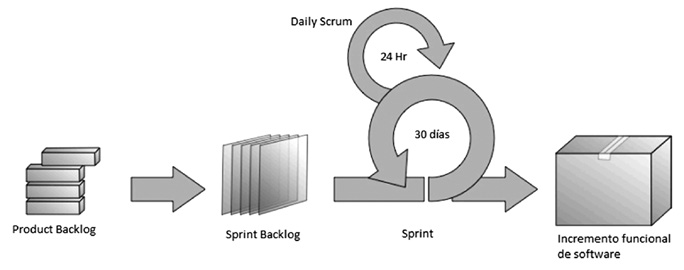
\includegraphics[width=11cm]{figuras/fasesDeUnSprint.png}}
    \caption{Ciclo de vida de un sprint}
    \label{fig::cicloDeVidaSprint}
\end{figure}

\begin{enumerate}
		\item \textbf{Planificación de la iteración (\textit{Sprint planning})}: se define el plan de trabajo de este Sprint especifico determinando qué se entregara y cómo se logrará. Es decir, se determinan las funcionalidades a implementar y la estimación de cantidad de trabajo. Con todo esto, y partiendo de la información en el \emph{Product backlog}, se establece el \emph{Sprint backlog}.
		\item \textbf{Reunión diaria (\textit{Daily meeting})}: cada día se realiza una reunión para explicar los objetivos que se han alcanzado desde la ultima reunión y determinar qué se realizará el día siguiente. Esto permite identificar problemas rápidamente y evitar que se retrase el ritmo de trabajo. \item \textbf{Revisión de la iteración (\emph{Sprint review})}: se realiza tras la finalización del Sprint completo. Se revisa todo lo que se hizo y lo que no, se comentan los problemas que tuvieron lugar y cómo se resolvieron, y se revisan los resultados obtenidos. 
		\item \textbf{Retrospectiva de la iteración (\emph{Sprint retrospective})}: esta reunión tiene el objetivo de analizar los puntos a mejorar y los puntos fuertes del equipo con el fin de aumentar la productividad.
		\item \textbf{Replanificación}: conjuntamente con el cliente se revisa la planificación teniendo en cuenta los posibles cambios que hayan podido surgir durante el \emph{Sprint}.
\end{enumerate}
			
\subsection{Aplicación de Scrum a este proyecto}
Dado que la mayoría de las practicas de Scrum están centradas en mejorar la productividad de un equipo, se han realizado una serie de adaptaciones teniendo en cuenta las características y circunstancias del proyecto. Se ha prescindido de la reunión diaria, pues el equipo de desarrollo está formado por una única persona. En este caso los sprints tuvieron una duración de inicial de 3 semanas, por lo que en lugar del \textit{Daily meeting} se ha optado por realizar una reunión semanal en la que se comentaba todo lo realizado hasta el momento y todas las actividades pendientes de abordar. Además, la reunión al final de cada sprint se realizó, en su mayoría, únicamente con los tutores y no con el cliente. Sin embargo, se mantuvo comunicación con este constantemente a lo largo de todo el desarrollo.

\subsection{DevOps}

Las antiguas metodologías de desarrollo de software separaban en dos sectores bien diferenciados aquellos que escribían el software (Dpto. Desarrollo) de aquellos que desplegaban en la nube (Dpto. Sistemas) \cite{devops5}.

DevOps surge con la idea de romper esta división y unir en un solo equipo a aquellos que desarrollan software y aquellos que lo despliegan. Esta unión proporciona transparencia a la hora de consultar el estado del producto y las distintas etapas que ha superado o superará.

La filosofía DevOps se basa en los mismos principios que las metodologías ágiles. Sin embargo, con DevOps se quiere fomentar una cultura de equipo, en la que todas las personas que formen el equipo sepan qué está haciendo cada una.

\subsubsection{Características de DevOps}
Esta filosofía busca la calidad de un producto software, creado por un equipo que se adapte rápido a los cambios e inconvenientes que aparezcan a lo largo de su desarrollo. Estos cambios deben ser identificados con rapidez para su posterior solución.

DevOps engloba todas las buenas prácticas a tener en cuenta a la hora de la entrega, el desarrollo y la administración de aplicaciones a lo largo del ciclo de vida de desarrollo de software: \cite{devops7}

\begin{itemize}
    \item Desarrollo y revisión de código con la ayuda de un controlador de versiones.
    \item Uso de herramientas de integración continua
    \item Continuo testeo del producto para obtener un software de calidad
    \item Uso de un gestor de repositorio optimizar la descarga y el almacenamiento de archivos binarios utilizados y producidos en el desarrollo de software.
    \item Uso de un gestor que automatice el proceso de despliegue
    \item Uso de un gestor de aprovisionamiento que nos cargue las configuraciones que necesarias de nuestro proyecto
    \item Monitorización del rendimiento de la aplicación
\end{itemize}

\subsection{Aplicación de DevOps a este proyecto}

Para este proyecto se usará Git \footnote{https://git-scm.com/} como herramienta para el control de versiones y GitHub \footnote{https://github.com/} como servicio público donde almacenar el repositorio de la aplicación.

Es fundamental en este proyecto el desarrollo basado en pruebas y la integración continua en el respositorio. El código debe de estar testeado previamente antes de añadirlo oficialmente al repositorio del mismo si se quiere obtener un software de calidad.

En este proyeco el equipo está formado por una persona, por lo que el mismo equipo será transparente y formado por el sector de desarrollo y el sector de despliegue.


\subsection{Combinación de Scrum y DevOps}

Como se ha explicado anteriormente, Scrum nos define un marco para el desarrollo de la aplicación. Un marco donde se definen Sprints para la consecución de objetivos.

Scrum se usará en este proyecto como una estructura que ayude a 

Dentro de cada Sprint, DevOps ayudará a la obtención de esos objetivos gracias a su filosofía, sobre todo su buena práctica relacionada en el desarrollo basado en pruebas, herramientas de automatización para el despliegue y la revisión del código gracias a un controlador de versiones.

\section{Gestión de la configuración}
En esta sección se define la gestión de la configuración bajo la cual desarrollaremos todas las actividades que impliquen la creación, modificación o eliminación de alguno de los elementos de trabajo que conforman este proyecto, asegurando así que todo lo que concierne al proyecto sea válido durante la vida del mismo.

 Teniendo en cuenta que los elementos de trabajo de este proyecto son los ficheros de código fuente y todos los archivos que conforman la documentación, abordaremos esta sección especificando, de forma independiente, cómo se ha tratado cada tipo de elemento de trabajo.
 
\subsection{Gestión del código}

Para la gestión del código se creará un repositorio local con un  sistema de control de versiones, que a su vez se sincronizará con un repositorio remoto en \textit{GitHub}, y por lo tanto almacenado en la nube. \textit{GitHub} es un servicio web de control de versiones y desarrollo de software basado en \textit{Git}, publicado bajo una Licencia de código abierto. Esta copia remota previene el riesgo de pérdida del código fuente.

\subsection{Gestión de la documentación}
Para almacenar la documentación de este proyecto se utilizará un repositorio en \textit{GitHub} llamado \textbf{Memoria\_TFG\_GuillermoMuriel} \footnote{https://github.com/guillesiesta/Memoria\_TFG\_GuillermoMuriel}.

Esta plataforma permite la creación de un repositorio cuyo lenguaje principal será LateX, y le añade una licencia de código abierto.

En cuanto a la edición y gestión de la memoria del proyecto, se utilizará la plataforma online \textit{Overleaf v2}\footnote{https://v2.overleaf.com/}. Dispone de control de versiones y edición en concurrencia. De la misma forma, al estar almacenada en la nube, se previene el riesgo de pérdida.

\section{Gestión del tiempo}
En este apartado se trata la planificación temporal del proyecto y las fases de la misma. Si bien se ha  establecido una planificación inicial, las tareas a realizar se especificarán de forma concreta a medida que se avance en el desarrollo del proyecto en función de los resultados obtenidos tras la finalización de cada sprint.

\subsection{Planificación de los sprints}

Teniendo en cuenta la metodología de desarrollo elegida, se ha optado por describir las tareas abordadas en cada sprint y su correspondiente gráfico \textit{Burn-Down}. Los diagramas \textit{Burn-down} son gráficos de dos ejes que se utilizan para representar el avance ideal del proyecto frente al avance real. En el eje X se representa el tiempo y en el eje Y la cantidad de trabajo. Es necesario actualizarlo diariamente. Antes, procederemos a introducir una visión general de los requisitos temporales escogidos sobre la organización del tiempo:

Disponemos de 300 horas para la realización del proyecto.

Para la realización de este proyecto se van a programar 5 sprints de 60 horas de duración cada uno. Por semana se trabajará de lunes a viernes unas 4 horas al día, en total 20 horas a la semana.

En total, se espera que cada sprint dure 3 semanas .

Por lo que el proyecto, salvo imprevisto, debería estar finalizado en torno a las 15 semanas. 

Aproximadamente debería concluir en 4 meses.

\begin{figure}[hbtp]
\begin{subfigure}{.5\textwidth}
    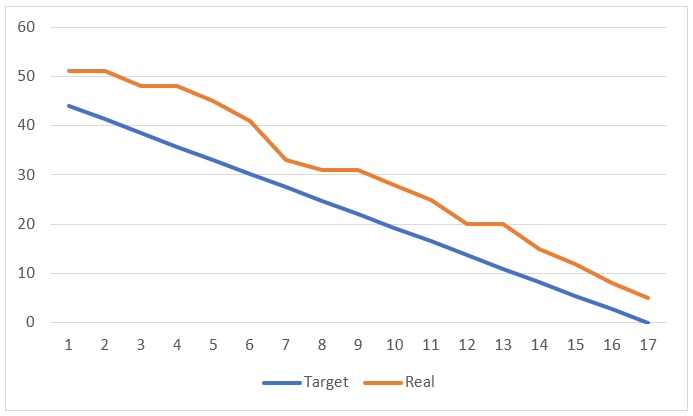
\includegraphics[width=\linewidth]{figuras/sprint1.png}
    \caption{Sprint 1}
    \label{fig:sprint1}
\end{subfigure}
\begin{subfigure}{.5\textwidth}
    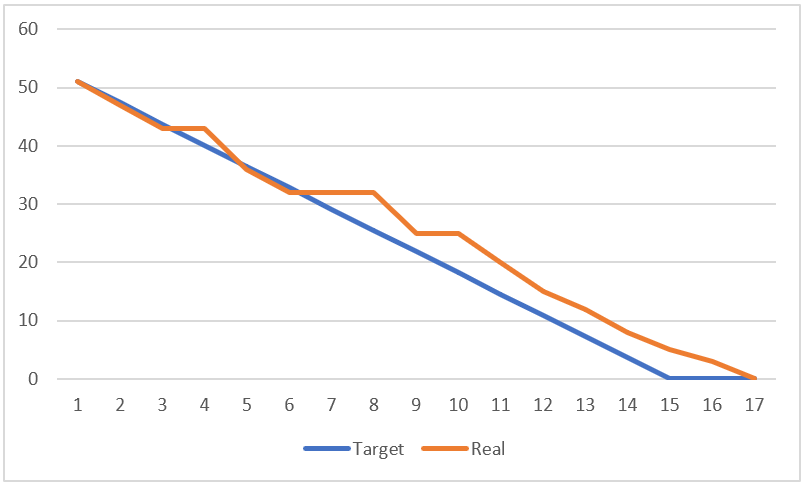
\includegraphics[width=\linewidth]{figuras/sprint2.png}
    \caption{Sprint 2}
    \label{fig:sprint2}
\end{subfigure}
\begin{subfigure}{.5\textwidth}
    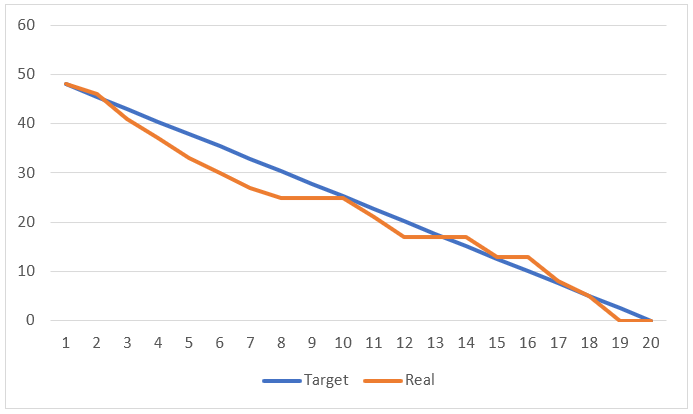
\includegraphics[width=\linewidth]{figuras/sprint3.png}
    \caption{Sprint 3}
    \label{fig:sprint3}
\end{subfigure}
\begin{subfigure}{.5\textwidth}
    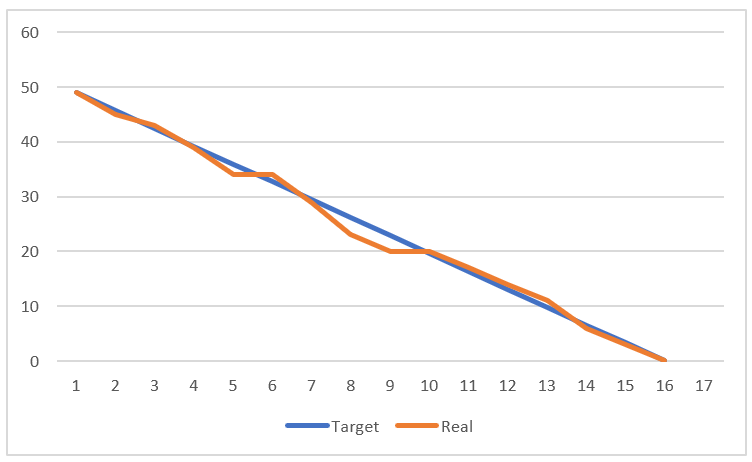
\includegraphics[width=\linewidth]{figuras/sprint4.png}
    \caption{Sprint 4}
    \label{fig:sprint4}
\end{subfigure}
\begin{subfigure}{\textwidth}
    \centering
    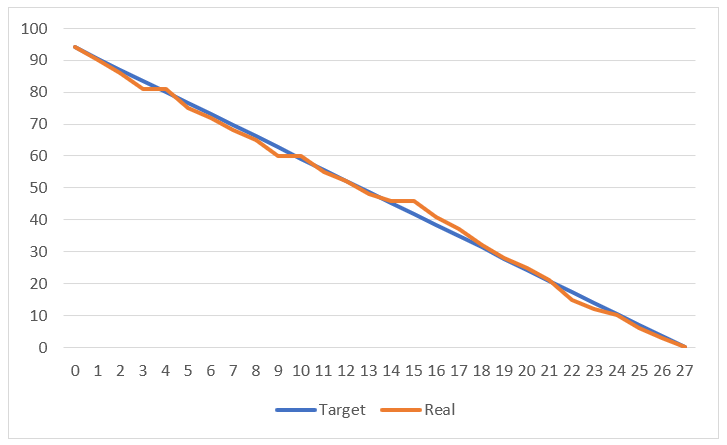
\includegraphics[width=.5\linewidth]{figuras/sprint5.png}
    \caption{Sprint 5}
    \label{fig:sprint5}
\end{subfigure}
\caption{Gráficos \textit{burn-down} de los distintos sprints del proyecto}
\label{fig:sprints}
\end{figure}

\begin{itemize}
    \item \textbf{Sprint 1}. En esta primera fase determinará la organización temporal y se estudiará la viabilidad del proyecto. Se extraerán los requisitos y a partir de estos se hará un análisis de las tecnologías existentes para poder desarrollar nuestro proyecto y desplegarlo en la nube y, se escogerán cuales serán las herramientas que más se adecúen a las necesidades del proyecto.
    
    \item \textbf{Sprint 2}. En esta segunda fase se comenzará a trabajar en el almacenamiento de datos, se extraerá toda la documentación necesaria y se procederá a la construcción de la misma. Nuestra base de datos debe estar organizada, estructurada y desarrollada para que en el siguiente sprint ya pueda ser utilizada.
    \item \textbf{Sprint 3}. En este sprint se procederá a construir nuestro intermediario entre la interfaz y la base de datos. Lo llamaremos controlador, es decir, nuestra API REST. Además, se implementaran tests que este controlador deberá de superar, así se confirma su correcto funcionamiento antes del montaje final. En esta fase conectaremos nuestro controlador a nuestra base de datos.
    \item \textbf{Sprint 4}. Esta fase está desarrollada única y enteramente al desarrollo de nuestra interfaz. Se escribirán los tests que deben de ser superados para que nuestra interfaz sea apta para su despliegue.
    \item \textbf{Sprint 5}. En la fase final se procederá a la unión de nuestra interfaz y nuestro controlador ya unido con la base de datos. A partir de aquí, con nuestro sistema funcionando y testeado, procederemos a desplegarlo usando las tecnologías escogidas previamente. 
    
    Una vez la aplicación esté desplegada, se procederá a la redacción de la memoria.
\end{itemize}

\section{Gestión de riesgos}
Un riesgo de un proyecto es un evento o condición  que podría tener un efecto positivo o negativo sobre alguno de los recursos u objetivos del proyecto, como podría ser tiempo, coste, alcance o calidad. La gestión de riesgos es un proceso continuo que debe considerar tanto fuentes internas como externas de dichos riesgos. Por norma general, la materialización de un riesgo implica consecuencias negativas, por lo que la gestión de riesgos tiene un papel muy importante dentro de la gestión del proyecto. 

En esta sección se identificarán los posibles riesgos del proyecto, estimando la probabilidad de aparición y su impacto potencial. Posteriormente se definirán las estrategias y pasos a seguir para prevenirlos o minimizar su impacto en caso de que se materialicen.

\subsection{Identificación de riesgos}
\begin{itemize}
\item \textbf{R001} - No identificar correctamente los requisitos del proyecto.
\item \textbf{R002} - Dificultad en las tareas de formación.
\item \textbf{R003} - Aparición de nuevos requisitos.
\item \textbf{R004} - No conseguir ajustar la planificación a las horas requeridas.
\item \textbf{R005} - Cambios en la planificación o retrasos en la misma.
\item \textbf{R006} - Errores eligiendo las tecnologías para el desarrollo del proyecto.
\item \textbf{R007} - Disponibilidad del experto insuficiente.
\item \textbf{R008} - La estructura de los datos de partida cambia con el tiempo.
\item \textbf{R009} - Nulo o deficiente proceso de validación y verificación .
\item \textbf{R010} - Detección de fallos importantes en el software tras la validación.
\item \textbf{R011} - Detección de fallos importantes en los resultados tras la validación.
\item \textbf{R012} - La interfaz no cumple con los requisitos.
\item \textbf{R013} - La API no cumple con los requisitos.
\item \textbf{R014} - La base de datos escogida no cumple con los requisitos.
\item \textbf{R015} - Pérdida de parte del proyecto (documentación o código).
\item \textbf{R016} - Computador de desarrollo estropeado.
\item \textbf{R017} - Se sobrepasan los límites de los servicios gratuitos de las plataformas escogidas.
\item \textbf{R018} - La plataforma GitHub no está disponible.
\item \textbf{R019} - Las tecnologías usadas cambian de versión durante el proceso de desarrollo.
\item \textbf{R020} - Problemas de transporte de información entre las tecnologías implementadas.
\end{itemize}

\subsection{Planificación de la respuesta a los riesgos}
\subsection{Riesgos materializados}

\section{Gestión de costes}
\subsection{Costes de recursos humanos}
\subsection{Costes de material}
\subsection{Costes de indirectos}
\subsection{Costes total del proyecto}



\chapter{Especificación de Requisitos}
Los requisitos se pueden definir como aquellas características esperables y/o deseables que debe cumplir un sistema para satisfacer unas necesidades especificas. Esta tarea es imprescindible para asegurar el éxito del proyecto. En esta sección describiremos los requisitos del proyecto desde una perspectiva menos tradicional que encaja mejor con la metodología de desarrollo elegida: historias de usuario. Las historias de usuario describen de forma breve aquello que un determinado usuario (en este caso desarrollador) espera al final del desarrollo. Es necesario que cumplan una serie de características:
\begin{itemize}
    \item Deben ser independientes.
    \item Ser negociables. No actúan como un contrato, sino como una serie de pautas de acción.
    \item Deben aportar valor al proyecto.
    \item Se debe poder realizar una estimación sobre ellas (temporal o de carga de trabajo).
    \item Deben tener un tamaño manejable.
    \item Deben ser verificables, pues es necesario saber si una historia se ha cumplido.
\end{itemize}

Cada historia se ha expresado siguiendo el siguiente patrón:
\begin{center}
    Como \texttt{<usuario>}, quiero / espero \texttt{<objetivo>}
\end{center}

Además cada una de ellas se acompaña de una estimación temporal, unos criterios de aceptación, un nivel de importancia y un identificador.

Se distinguirán entre tres tipos de niveles de importancia, según su prioridad.
\begin{itemize}
    \item \textbf{Alta} (Cumplimiento obligatorio): la historia es imprescindible para el desarrollo y éxito del proyecto. Es necesario que esté en la versión final para aceptar el proyecto.
    \item \textbf{Media} (Cumplimiento deseable): es deseable la presencia de esta historia en la versión final del proyecto, pero no supone un aumento significativo del valor del producto.
    \item \textbf{Baja} (Cumplimiento opcional): su presencia no es crucial para el éxito del proyecto, pero aporta cierto valor funcional. 
\end{itemize}

Aún cuando el tiempo total de todas las historias de usuario sea mayor al tiempo disponible, no supone un inconveniente, pues las historias se desarrollarán más de una a la vez ya que se solapan y es casi imposible determinar tareas aisladas para el cumplimiento de cada una.

A continuación se especificarán todas las historias de usuario del proyecto teniendo en cuenta el  documento guía \ref{tab:HC-EJEMPLO} para la especificación de historias de usuario.

\begin{table}[htbp]
\centering
\begin{tabular}{|c|L{10.5cm}|}
    \hline
    \multicolumn{2}{|l|}{\textbf{Código} - Nombre} \\\hline 
    \textbf{Descripción}	&  Breve descripción de la historia de usuario. \\\hline
    \textbf{Estimación}	&	Estimación temporal de la historia. 	\\\hline
    \textbf{Prioridad}	&	Prioridad según la importancia que tiene esta historia para el desarrollo satisfactorio del proyecto.	\\\hline
    \textbf{Aceptación}	&	Criterios a cumplir para considerar que esta historia de usuario se ha cubierto satisfactoriamente.		\\\hline
    \textbf{Notas}		&	Observaciones varias.		\\\hline
\end{tabular}
\caption{Documento guía. Especificación de las historias de usuario.}
\label{tab:HC-EJEMPLO}
\end{table}

\section{Historias de usuario}

\begin{table}[H]
\centering
\label{tab:HU-0}
\begin{tabular}{|c|L{10.5cm}|}
    \hline
    \multicolumn{2}{|l|}{\textbf{HU-00} -Proponer una solución a un acertijo} \\\hline 	
    \textbf{Descripción}	& Quiero que el usuario sea capaz de proponer soluciones a los acertijos del sistema
	\\\hline
    \textbf{Estimación}	&	3 semanas	\\\hline
    \textbf{Prioridad}	&	Alta		\\\hline
    \textbf{Aceptación}	&	En el caso de que el usuario introduzca correctamente una solución a un acertijo, ésta se almacenará en la plataforma y se enlazará con el acertijo	\\\hline
    \textbf{Notas}		&			\\\hline
\end{tabular}
\end{table}

\begin{table}[H]
\centering
\label{tab:HU-1}
\begin{tabular}{|c|L{10.5cm}|}
    \hline
    \multicolumn{2}{|l|}{\textbf{HU-01} - Login o acceso a la aplicación} \\\hline 	
    \textbf{Descripción}	& Quiero que el usuario acceda a la plataforma a través de usuario y contraseña
	\\\hline
    \textbf{Estimación}	&	3 semanas	\\\hline
    \textbf{Prioridad}	&	Alta		\\\hline
    \textbf{Aceptación}	&	En el caso de que el usuario introduzca correctamente su usuario y contraseña, se accederá a la plataforma	\\\hline
    \textbf{Notas}		&			\\\hline
\end{tabular}
\end{table}

\begin{table}[H]
\centering
\label{tab:HU-2}
\begin{tabular}{|c|L{10.5cm}|}
    \hline
    \multicolumn{2}{|l|}{\textbf{HU-02} - Escribir un acertijo} \\\hline 	
    \textbf{Descripción}	& Quiero que el usuario sea capaz de escribir un acertijo y subirlo a la plataforma
	\\\hline
    \textbf{Estimación}	&	3 semanas	\\\hline
    \textbf{Prioridad}	&	Alta		\\\hline
    \textbf{Aceptación}	&	Cuando el usuario introduzca su acertijo, éste deberá ser accesible en la plataforma	\\\hline
    \textbf{Notas}		&			\\\hline
\end{tabular}
\end{table}

\begin{table}[H]
\centering
\label{tab:HU-3}
\begin{tabular}{|c|L{10.5cm}|}
    \hline
    \multicolumn{2}{|l|}{\textbf{HU-03} - Consulta de propios acertijos} \\\hline 	
    \textbf{Descripción}	& Quiero que el usuario sea capaz de consultar el estado de sus acertijos
	\\\hline
    \textbf{Estimación}	&	3 semanas	\\\hline
    \textbf{Prioridad}	&	Media		\\\hline
    \textbf{Aceptación}	&	Cuando el usuario introduzca su acertijo, éste deberá ser accesible en la plataforma en un apartado en que solamente se muestren los acertijos escritos del usuario	\\\hline
    \textbf{Notas}		&			\\\hline
\end{tabular}
\end{table}

\begin{table}[H]
\centering
\label{tab:HU-4}
\begin{tabular}{|c|L{10.5cm}|}
    \hline
    \multicolumn{2}{|l|}{\textbf{HU-04} - Puntuación de las respuestas de un acertijo} \\\hline 	
    \textbf{Descripción}	& Quiero que el usuario sea capaz de puntuar las respuestas propuestas por los demás usuarios sobre sus acertijos
	\\\hline
    \textbf{Estimación}	&	3 semanas	\\\hline
    \textbf{Prioridad}	&	Alta		\\\hline
    \textbf{Aceptación}	&	Cuando el usuario acceda a las soluciones del acertijo y modifique la puntuación de la solución, ésta deberá ser actualizada al momento.	\\\hline
    \textbf{Notas}		&			\\\hline
\end{tabular}
\end{table}

\begin{table}[H]
\centering
\label{tab:HU-5}
\begin{tabular}{|c|L{10.5cm}|}
    \hline
    \multicolumn{2}{|l|}{\textbf{HU-05} - Actualización del porcentaje del estado de un acertijo } \\\hline 	
    \textbf{Descripción}	& Quiero que sistema actualice el estado de un acertijo basándose en las puntuaciones obtenidas de las respuestas propuestas al mismo
	\\\hline
    \textbf{Estimación}	&	3 semanas	\\\hline
    \textbf{Prioridad}	&	Alta		\\\hline
    \textbf{Aceptación}	&	Cuando el usuario acceda a un acertijo, éste mostrará el estado de resolución en el que se encuentra	\\\hline
    \textbf{Notas}		&			\\\hline
\end{tabular}
\end{table}

\begin{table}[H]
\centering
\label{tab:HU-6}
\begin{tabular}{|c|L{10.5cm}|}
    \hline
    \multicolumn{2}{|l|}{\textbf{HU-06} - Consulta de todas las soluciones propuestas a un acertijo } \\\hline 	
    \textbf{Descripción}	& Quiero que un usuario al acceder a un acertijo a resolver, tenga la posibilidad de consultar todas las propuestas como solución escritas para el mismo
	\\\hline
    \textbf{Estimación}	&	3 semanas	\\\hline
    \textbf{Prioridad}	&	Alta		\\\hline
    \textbf{Aceptación}	&	Al acceder a un acertijo, si éste tiene soluciones, deberán mostrarse en el caso de que el usuario lo solicite 	\\\hline
    \textbf{Notas}		&			\\\hline
\end{tabular}
\end{table}

\begin{table}[H]
\centering
\label{tab:HU-7}
\begin{tabular}{|c|L{10.5cm}|}
    \hline
    \multicolumn{2}{|l|}{\textbf{HU-07} -Modificación de los datos de un usuario } \\\hline 	
    \textbf{Descripción}	& Quiero que un usuario pueda modificar sus datos
	\\\hline
    \textbf{Estimación}	&	3 semanas	\\\hline
    \textbf{Prioridad}	&	Baja		\\\hline
    \textbf{Aceptación}	&	Al acceder a sus datos personales y modificarlos, éstos se actualizarán automáticamente en el sistema 	\\\hline
    \textbf{Notas}		&	Esta funcionalidad se contemplará única y exclusivamente cuando se disponga de tiempo de más en el sprint correspondiente		\\\hline
\end{tabular}
\end{table}


\begin{table}[H]
\centering
\label{tab:HU-8}
\begin{tabular}{|c|L{10.5cm}|}
    \hline
    \multicolumn{2}{|l|}{\textbf{HU-08} - Adaptabilidad a distintos front-ends } \\\hline 	
    \textbf{Descripción}	& Quiero que mi aplicación sea adaptable a distintos front-end
	\\\hline
    \textbf{Estimación}	&	3 semanas	\\\hline
    \textbf{Prioridad}	&	Alta		\\\hline
    \textbf{Aceptación}	&	La API desarrollada debe de ser accesible desde cualquier lugar y en cualquier momento. Esto es, debe permitir el acceso a peticiones HTTP. 	\\\hline
    \textbf{Notas}		&			\\\hline
\end{tabular}
\end{table}

\begin{table}[H]
\centering
\label{tab:HU-10}
\begin{tabular}{|c|L{10.5cm}|}
    \hline
    \multicolumn{2}{|l|}{\textbf{HU-10} - Interfaz sencilla e intuitiva } \\\hline 	
    \textbf{Descripción}	& Quiero que mi aplicación sea fácil de usar y atractiva
	\\\hline
    \textbf{Estimación}	&	3 semanas	\\\hline
    \textbf{Prioridad}	&	Alta		\\\hline
    \textbf{Aceptación}	&	La interfaz no contendrá excesiva carga de información, y será intuitiva 	\\\hline
    \textbf{Notas}		&			\\\hline
\end{tabular}
\end{table}

\begin{table}[H]
\centering
\label{tab:HU-11}
\begin{tabular}{|c|L{10.5cm}|}
    \hline
    \multicolumn{2}{|l|}{\textbf{HU-11} - Accesibilidad y gestión de los datos } \\\hline 	
    \textbf{Descripción}	& Quiero que la base de datos de mi aplicación sea sencilla de administrar y que acepte peticiones HTTP de mi API
	\\\hline
    \textbf{Estimación}	&	3 semanas	\\\hline
    \textbf{Prioridad}	&	Alta		\\\hline
    \textbf{Aceptación}	&	La base de datos no dispondrá de excesiva complejidad y será accesible, alojándose ésta en la nube 	\\\hline
    \textbf{Notas}		&			\\\hline
\end{tabular}
\end{table}

\begin{table}[H]
\centering
\label{tab:HU-12}
\begin{tabular}{|c|L{10.5cm}|}
    \hline
    \multicolumn{2}{|l|}{\textbf{HU-12} - Tecnologías usadas libres } \\\hline 	
    \textbf{Descripción}	& Quiero desarrollar mi aplicación con software libre
	\\\hline
    \textbf{Estimación}	&	3 semanas	\\\hline
    \textbf{Prioridad}	&	Media		\\\hline
    \textbf{Aceptación}	&	La mayor parte de la aplicación deberá estar desarrollada con software libre 	\\\hline
    \textbf{Notas}		&			\\\hline
\end{tabular}
\end{table}

\chapter{Análisis}
En este capítulo se aborda la fase de análisis de los distintos requerimientos  del sistema para cumplir con los objetivos del proyecto. 
La tarea principal será cumplir estos requerimientos de la manera más eficaz posible.
\section{Requisitos de la aplicación}
\section{Tecnologías a emplear}

\chapter{Diseño e Implementación}

\section{Arquitectura Cliente-Servidor}

El proyecto en general está basado en la arquitectura cliente-servidor\cite{clienteservidor}. Esta arquitectura define dos roles principales que se reparten tareas de demanda y respuesta, éstos respectivamente son:

\begin{itemize}
    \item Cliente
    \item Servidor
\end{itemize}

Esta separación se produce en nuestro proyecto cuando distinguimos entre front-end (cliente) y nuestro back-end (servidor).

Nuestra interfaz haría las funciones de cliente, sería la demandante de información y nuestra API junto con la base de datos sería nuestro servidor y encargado de procesar las peticiones y responder de manera adecuada a la petición original.

Con esta disposición disponemos de la ventaja que al tener bien diferenciado el back-end, nuestra aplicación será adaptable a cualquier tipo de front-end.

La función de mantenimiento es mucho más fácil de llevar a cabo en este tipo de arquitecturas, pues si aparece algún problema en la parte de interfaz, se puede corregir sin que la corrección aplicada altere el funcionamiento de nuestro back-end o API.

\subsection{Arquitectura Cliente-Servidor y Modelo Vista Controlador}

Estas dos arquitecturas no son incompatibles, en este proyecto se han diferenciado basándonos en el MVC 3 bloques distintos con funciones asignadas: vista, controlador y modelo. 

Una vez desarrollados esos bloques, la arquitectura cliente servidor engloba en un solo bloque, llamado servidor a los bloques: controlador y modelo. La función que esta arquitectura entiende por servidor es la que se realizaría gracias a la unión de estos dos bloques.

\section{Diseño}

El diseño es un proceso que permite construir una representación abstracta del software de forma que se puedan conocer aspectos como la arquitectura, funcionalidades o la calidad antes de comenzar la codificación. Además, permite detectar problemas en etapas muy tempranas del proyecto, ahorrando costes y reduciendo la presencia de riesgos. En Scrum el diseño del software es continuo y se actualiza en cada sprint.

A continuación se mencionan algunos aspectos del diseño de la aplicación que resultan interesantes o relevantes para el correcto funcionamiento.

\subsection{Representación de los datos}

Los datos serán representados en nuestro bloque o módulo que actuará como vista. Para ello, como ya describimos en la fase de análisis, lo desarrollaremos usando el framework ReactJS.

Estos datos tienen que mostrarse en una interfaz que sea sencilla de usar, intuitiva y que se adapte a todo tipo de navegadores. 

Para la elección del aspecto de la misma, es necesaria la búsqueda de inspiración. Por lo que la interfaz de la aplicación Instagram\footnote{https://www.instagram.com/?hl=es} ha sido considerada el modelo a seguir. Observando esta interfaz en la figura \ref{fig::insta}, se puede comprobar que en cualquier momento, un usuario tiene la posibilidad de cambiar la vista general gracias a los 4 botones que contiene en el extremo inferior de la pantalla. Esta funcionalidad, será clave a la hora de buscar una plantilla que ayude para el inicio del desarrollo de nuestra interfaz. Pues, en nuestro diseño será fundamental que el usuario tenga la posibilidad de desplazarse por los distintos apartados de la aplicación siempre que lo necesite.

\begin{figure}[htbp]
    \centerline{
\includegraphics[width=4cm]{figuras/insta.jpg}}
    \caption{Interfaz de Instagram}
    \label{fig::insta}
\end{figure}

La idea principal es la reutilización de código con licencia de código abierto. Gracias a la comunidad de software libre, se ha encontrado una interfaz que relacione la idea descrita anteriormente junto con un diseño sencillo e intuitivo. Esta plantilla se llama \textit{adminLTE}\footnote{https://github.com/almasaeed2010/AdminLTE}, está liberada bajo la licencia de software libre \textit{MIT}\footnote{https://github.com/almasaeed2010/AdminLTE/blob/master/LICENSE} y se encuentra alojada en la plataforma GitHub.

Gracias al uso de la misma, se ha podido desarrollar una interfaz sencilla de desarrollar y agradable a la vista. En la imagen \ref{fig::rid} se puede observar como se ha desarrollado una interfaz en la que un usuario puede, en cualquier momento cambiar el contenido de la vista principal.

\begin{figure}[htbp]
    \centerline{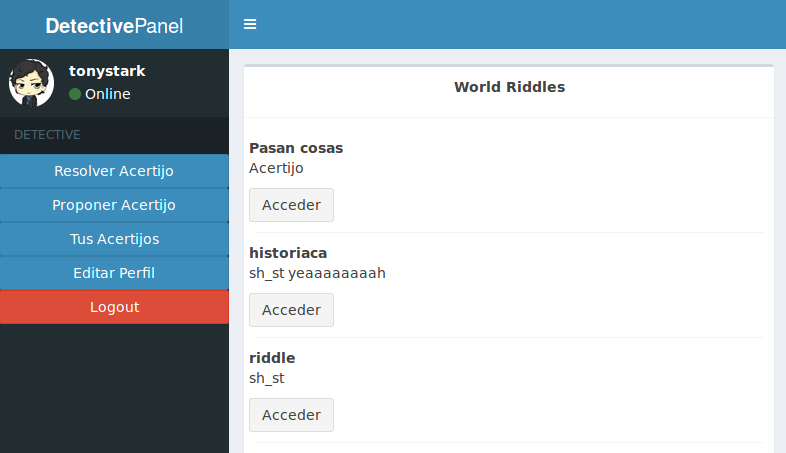
\includegraphics[width=12cm]{figuras/riddling.png}}
    \caption{Interfaz de Riddling, nuestro proyecto}
    \label{fig::rid}
\end{figure}

\subsubsection{ReactJS y sus componentes}

ReactJS es un framework que se basa en la reutilización de componentes. Un componente es cualquier estructura definida en la que se mostrará información. Cada componente se comporta como una instancia de una clase, por lo que cada uno de ellos tiene sus atributos definidos.

El procedimiento a seguir para la creación de la vista ha sido la creación y desarrollo de las 4 vistas iniciales que dispondrá nuestra aplicación:

\begin{itemize}
    \item \textbf{AcertijosView}. En este apartado se mostrarán todas las historias accesibles del sistema. Esta vista contendrá todos los componentes \textit{SmallRiddle} que posteriormente describiremos. Esta vista se puede observar en la figura \ref{fig::acertijosview}.
    \item \textbf{ProponerView}. En este apartado se mostrará un formulario para que un usuario introduzca un acertijo. Esta vista se puede observar en la figura \ref{fig::proponerview}.
    \item \textbf{TusAcertijosView}. En este apartado se mostrarán todas las historias propias de un usuario. Esta vista también contendrá todos los componentes \textit{SmallRiddle} que posteriormente describiremos. Esta vista se puede observar en la figura \ref{fig::tusacertijosview}.
    \item \textbf{EditarPerfilView}. Gracias a esta vista un usuario será capaz de administrar su perfil. Aparecerá un formulario con los datos que podrá modificar. Nótese que esta interfaz se encuentra diseñada pero actualmente se encuentra sin funcionalidad. Se puede observar en la figura \ref{fig::editarperfilview}.
\end{itemize}

\begin{figure}[hbtp] \centering
\begin{subfigure}{.6\textwidth}
    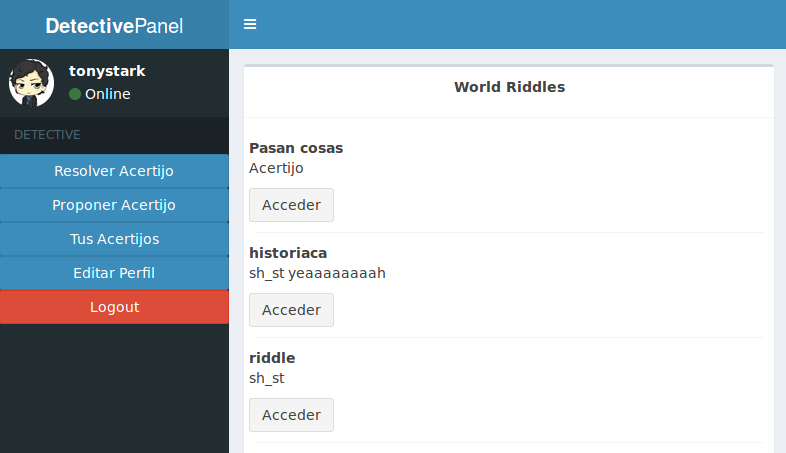
\includegraphics[width=\linewidth]{figuras/riddling.png}
    \caption{Vista AcertijosView de nuestra aplicación}
    \label{fig::acertijosview}
\end{subfigure}
\begin{subfigure}{.6\textwidth}
    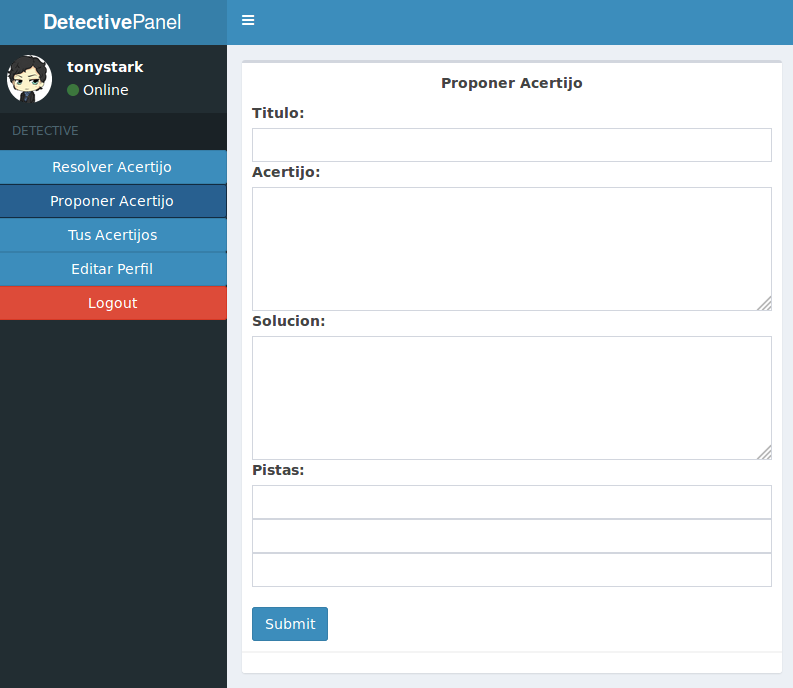
\includegraphics[width=\linewidth]{figuras/proponerview.png}
    \caption{Vista ProponerView de nuestra aplicación}
    \label{fig::proponerview}
\end{subfigure}

\begin{subfigure}{.6\textwidth}
    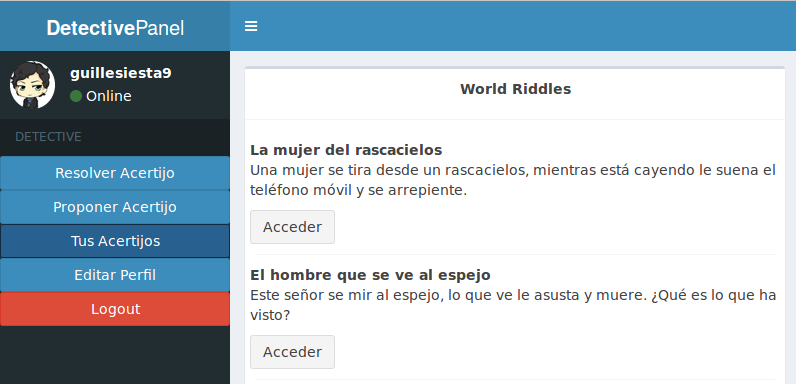
\includegraphics[width=\linewidth]{figuras/tusacertijosview.png}
    \caption{Vista de TusAcertijosView de nuestra aplicación}
    \label{fig::tusacertijosview}
\end{subfigure}

\begin{subfigure}{.6\textwidth}
    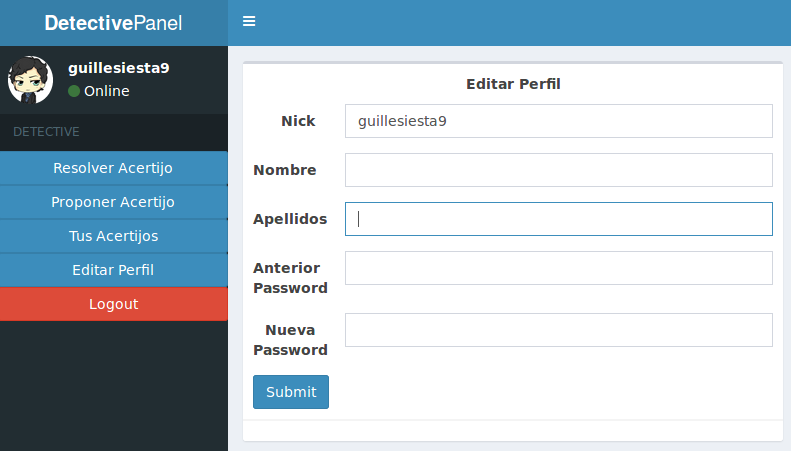
\includegraphics[width=\linewidth]{figuras/editarperfilview.png}
    \caption{Vista de EditarPerfilView de nuestra aplicación} 
    \label{fig::editarperfilview}
\end{subfigure}
\caption{Imágenes de las vistas que componen la aplicación}
\label{fig::vistas}
\end{figure}

Una vez definidas las vistas, éstas contendrán distintos tipos de componentes, que interactuarán entre ellos para poder realizar las funciones descritas en los requisitos de nuestra aplicación. Estos componentes se dividen en:

\begin{itemize}
    \item \textbf{Header}. En este componente encontramos la cabecera de la aplicación. Contiene un botón que al pulsarlo contrae hacia la izquierda el menú Sidebar. Está siempre renderizado.
    \item \textbf{Sidebar}. Este componente es el encargado de seleccionar qué vista es la que queremos escoger y visualizar. Este component se encuentra siempre accesible.
    \item \textbf{FormLogin}. El componente inicial que nos permite acceder a la plataforma.
    \item \textbf{SmallRiddle}. Es un componente que resume el título del acertijo y la descripción del mismo. Tenemos la posibilidad de acceder a él para así cargar el componente Riddle.
    \item \textbf{Riddle}. Muestra todos los datos del acertijo, a excepción de la solución. Este componente nos permite observar el estado en el que se encuentra el acertijo, la descripción del mismo, y las 3 valiosas pistas que nos ayudarán a resolverlo.
    
    Como funcionalidad adicional, este componente puede cargar todas las soluciones de ese acertijo propuestas por los usuarios y el porcentaje de cercanía con respecto a la solución final.
    \item \textbf{Solucion}. Componente que muestra el texto de la propuesta como solución de un acertijo y la puntuación otorgada por el creador del acertijo.
    \item \textbf{SolucionConCheck}. Este componente muestra la solución de un acertijo en concreto, y tiene la posibilidad de poder establecer una puntuación con respecto al porcentaje de cercanñia a la solución del acertijo. Este componente se renderiza úncamente en la vista TusAcertijosView.
\end{itemize}

En los bloques de figuras \ref{fig::componentes} y \ref{fig::componentes2} se puede observar el aspecto de cada uno de los componentes descritos.

\begin{figure}[hbtp] \centering
\begin{subfigure}{.6\textwidth}
     \centerline{
\includegraphics[width=8cm]{figuras/header.png}}
    \caption{Componente Header de nuestra aplicación}
    \label{fig::header}
\end{subfigure}
\begin{subfigure}{.6\textwidth}
    \centerline{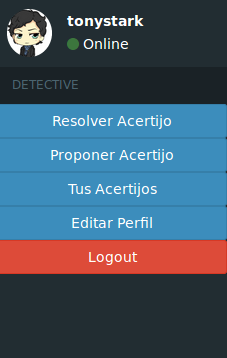
\includegraphics[width=5cm]{figuras/sidebar.png}}
    \caption{Componente Sidebar de nuestra aplicación}
    \label{fig::sidebar}
\end{subfigure}

\begin{subfigure}{.6\textwidth}
     \centerline{
\includegraphics[width=9cm]{figuras/smallriddle.png}}
    \caption{Componente SmallRiddle de nuestra aplicación}
    \label{fig::smallriddle}
\end{subfigure}
\caption{Imágenes de los componentes que componen la aplicación}
\label{fig::componentes}
\end{figure}


\begin{figure}[hbtp] \centering
\begin{subfigure}{.6\textwidth}
     \centerline{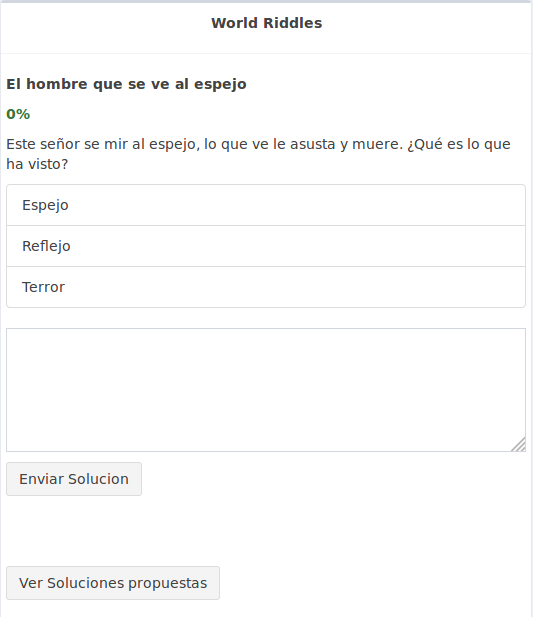
\includegraphics[width=9cm]{figuras/riddle.png}}
    \caption{Componente Riddle de nuestra aplicación} 
    \label{fig::riddle}
\end{subfigure}
\begin{subfigure}{.6\textwidth}
     \centerline{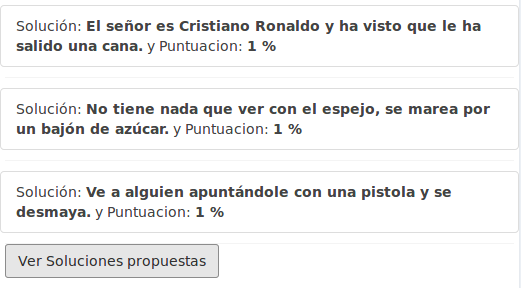
\includegraphics[width=9cm]{figuras/solucion.png}}
    \caption{Componente Solución de nuestra aplicación} 
    \label{fig::solucion}
\end{subfigure}

\begin{subfigure}{.6\textwidth}
     \centerline{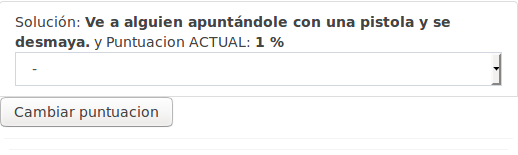
\includegraphics[width=9cm]{figuras/solucionconcheck.png}}
    \caption{Componente SoluciónConCheck de nuestra aplicación} 
    \label{fig::solucionconcheck}
\end{subfigure}
\caption{Imágenes de los componentes que componen la aplicación}
\label{fig::componentes2}
\end{figure}


\subsection{Modulado de los datos}

En esta aplicación se van a 2 distinguir dos tipos de entidades:

\begin{itemize}
    \item  Usuarios.
    \item  Acertijos.
\end{itemize}

Esto, traducido a nuestra base de datos basada en grafos, lo que estamos definiendo son 2 tipos de nodos específicos.

\begin{itemize}
    \item  \textbf{Usuarios}.
    \item  \textbf{Storie}.
\end{itemize}

Se representan en la base de datos de la la forma que muestra el bloque de imágenes \ref{fig::nodos}

\begin{figure}[hbtp] \centering
\begin{subfigure}{.6\textwidth}
     \centerline{
\includegraphics[width=2cm]{figuras/usuario.png}}
    \caption{Nodo Usuario} 
    \label{fig::riddle}
\end{subfigure}
\begin{subfigure}{.6\textwidth}
     \centerline{
\includegraphics[width=2cm]{figuras/storie.png}}
    \caption{Nodo Storie} 
    \label{fig::solucion}
\end{subfigure}
\caption{Nodos de nuestra base de datos }
\label{fig::nodos}
\end{figure}

\subsubsection{Atributos del usuario}

En la base de datos se almacenarán esta serie de atributos por nodo usuario:

\begin{itemize}
    \item \textbf{Nick}.
    \item \textbf{Contraseña}.
    \item \textbf{Nombre}.
    \item \textbf{Apellidos}.
\end{itemize}


\subsubsection{Atributos del acertijo}
En nuestra base de datos se almacenarán esta serie de atributos por nodo storie:

\begin{itemize}
    \item \textbf{Título}.
    \item \textbf{Sh\_Storie}. (acertijo)
    \item \textbf{Storie}. (solución)
    \item \textbf{Pista 1}.
    \item \textbf{Pista 2}.
    \item \textbf{Pista 3}.
\end{itemize}

\subsubsection{Relaciones entre nodos}

En el sistema se distinguen 2 tipos de relaciones:

\begin{itemize}
    \item \textbf{Escribe}. Relacionará cuando un usuario escribe un acertijo.
    \item \textbf{Propone}. Relacionará cuando un usuario propone una solución a un acertijo.
\end{itemize}

Una vez se establece el tipo de relaciones existentes en el sistema y se decida crear una relación \textit{Usuario escribe historia}, la representación gráfica sería la siguiente que se muestra en la figura \ref{fig::escribe}.

\begin{figure}
     \centerline{
\includegraphics[width=5cm]{figuras/escribe.png}}
    \caption{Relación (Usuario)-[Escribe]-(Storie)} 
    \label{fig::escribe}
\end{figure}

Neo4j nos ofrece la posibilidad de poder añadir atributos a las relaciones. Esto será útil para la relación \textit{propone}, pues en esa relación será necesario registrar el texto propuesto como solución y la puntuación de esa propuesta (inicialmente será de 1).

Esta relación quedaría representada tal y como describe la figura \ref{fig::propone}.

\begin{figure}
     \centerline{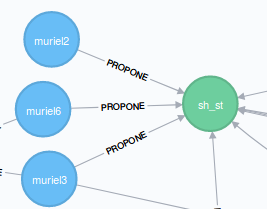
\includegraphics[width=5cm]{figuras/propone.png}}
    \caption{Relación (Usuario)-[Propone]-(Storie)} 
    \label{fig::propone}
\end{figure}

\subsubsection{Conclusión sobre el modelado de grafos y su consulta}

Como se puede observar, es realmente intuitiva y sencilla la representación gráfica que este tipo de base de dato nos propone.

Sin embargo, más sencillo  en intuitivo es aún el lenguaje \textit{Cypher} necesario para la realización de consultas. Pues éste, con una breve ojeada a su manual de usuario\footnote{https://neo4j.com/docs/developer-manual/current/cypher/}, ya se es capaz de realizar cualquier tipo de consulta necesaria para el funcionamiento de la aplicación. Por ejemplo, en el caso de que necesitáramos extraer de la base de datos todos los acertijos propuestos por el usuario "aristoteles", la consulta sería la siguiente:

\textit{MATCH (u:Usuario)-[r:Escribe]-(s:Storie) WHERE u.nick=aristoteles RETURN s.storie}

\subsection{Control de los datos}

Esta aplicación tiene que garantizar la seguridad de que todos los datos enviados y recibidos por los componentes o la base de datos son gestionados de manera adecuada. Es para ello que nuestro controlador necesitará de unos métodos a los que llamar desde nuestra interfaz.

Este controlador deberá de estar conectado a nuestra base de datos, y tendrá que ser apto al recibo de peticiones por parte de la interfaz. Nuestro controlador deberá limitarse única y exclusivamente a la ejecución de esos métodos, por lo que necesitamos que sea un sericio ligeo. Flask nos garantiza todo lo anterior.

Nuestro controlador tendrá los siguientes métodos:

\begin{itemize}
    \item \textbf{all\_stories\_titulo()}. Se devuelven todos los títulos de las historias del sistema.
    \item \textbf{user\_stories\_titulo()}. Se devuelven los títulos de las historias creadas por un usuario en concreto.
    \item \textbf{soluciones\_por\_titulo()}. Se devuelven de un acertijo todas las soluciones propuestas y su puntuación.
    \item \textbf{enviar\_comentario()}. Se añade en la base de datos la propuesta de solución de un usuario para un acertijo en concreto.
    \item \textbf{enviar\_storie()}. Se añade en la base de datos un acertijo.
    \item \textbf{cambiar\_puntuacion\_titulo()}. Se modifica en la base de datos la puntuación de una posible solución de un acertijo. Una vez cambiada la puntuación, se procederá a la actualización del estado del acertijo buscando cual es la mayor puntuación que existe de las soluciones propuestas. Esta puntuación pasará a ser el mayor de puntuación de cualquier propuesta de solución.
    \item \textbf{acertijo\_por\_titulo()}. Se busca en la base de datos el acertijo que coincida con ese título y se devuelve el texto del mismo.
    \item \textbf{storie\_por\_titulo()}. Se busca en la base de datos el acertijo que coincida con ese título y se devuelve la solución del mismo.
    \item \textbf{todo\_por\_titulo()}. Se busca en la base de datos un acertijo a partir de su título y se devuelven todos sus atributos.
    \item \textbf{login()}. Se busca en la base de datos si el usuario existe y la contraseña coincide con la registrada en el sistema.
\end{itemize}

\subsection{Flujo de los datos}

El flujo de datos puede ir desde nuestra interfaz hasta nuestra base de datos y viceversa. Para que esto ocurra, necesitamos nuestro controlador como intermediario. 

El formato de los datos estará estructurado en JSON\footnote{https://www.json.org/}, debido a su alto uso en peticiones y respuestas mediante el protocolo HTTP.

Esto es, en el caso de que desde nuestra interfaz, decidamos añadir nuestro acertijo creado, se enviará en formato JSON los datos al controlador, que extraerá la información relevante de ese JSON y añadirá lo especificado a la base de datos.

Un ejemplo de flujo de datos y pasos a seguir puede ser el ejemplo descrito en los diagramas de secuencia \ref{fig::secuencia}. En estos diagrama, se describe el funcionamiento de los eventos \textit{enviar\_storie(), enviar\_comentario(),}, en el que un usuario introduce un nuevo acertijo en el sistema.

\begin{figure}[hbtp] \centering
\begin{subfigure}{.6\textwidth}
     \centerline{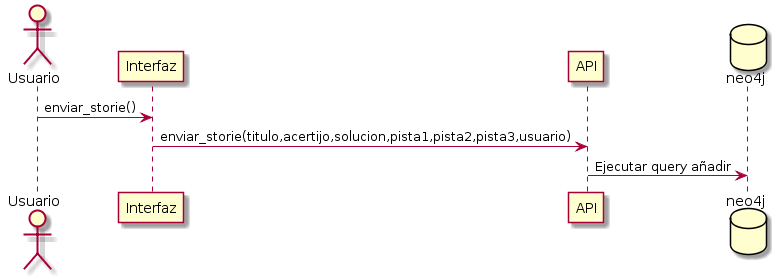
\includegraphics[width=11cm]{figuras/enviar_storie.png}}
    \caption{Diagrama de secuencia del evento enviar\_storie()} 
    \label{fig::enviarstorie}
\end{subfigure}
\begin{subfigure}{.6\textwidth}
     \centerline{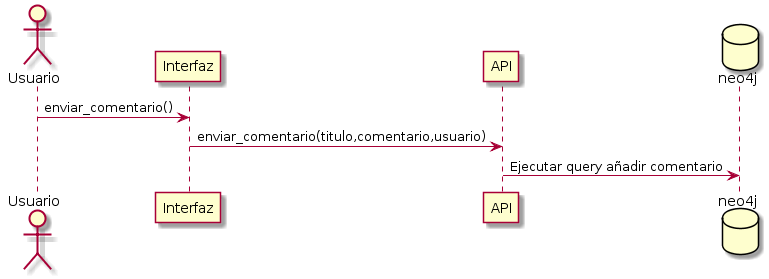
\includegraphics[width=11cm]{figuras/enviar_comentario.png}}
    \caption{Diagrama de secuencia del evento enviar\_comentario()} 
    \label{fig::enviarcomentario}
\end{subfigure}
\begin{subfigure}{.6\textwidth}
     \centerline{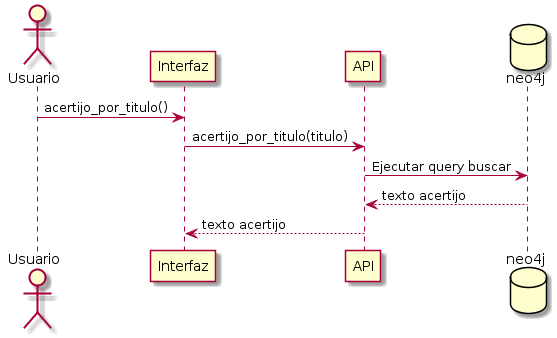
\includegraphics[width=11cm]{figuras/acertijo_por_titulo.png}}
    \caption{Diagrama de secuencia del evento acertijo\_por\_titulo()} 
    \label{fig::acertijoportitulo}
\end{subfigure}
\begin{subfigure}{.6\textwidth}
     \centerline{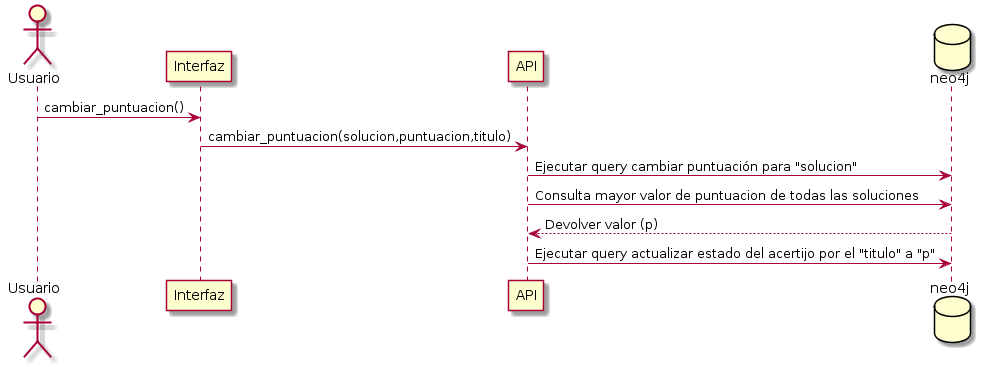
\includegraphics[width=11cm]{figuras/cambiar_puntuacion.png}}
    \caption{Diagrama de secuencia del evento cambiar\_puntuacion()} 
    \label{fig::cambiarpuntuacion}
\end{subfigure}
\caption{Diagramas de flujo de algunos eventos de la aplicación }
\label{fig::secuencia}
\end{figure}


\section{Implementación}

Una vez descrito el funcionamiento de la aplicación, el siguiente paso es la implementación. Se distinguen dos fases a la hora de llevar a cabo esta etapa. Seguiremos el orden de una primera fase en la que se desarrolla la aplicación en nuestra computadora local y otra segunda, en la que se desarrollan los automatismos necesarios para el despliegue de la aplicación creada en local.

\subsection{Implementación en local}

Para la implementación de la aplicación en local se han implementado los 3 bloques de una manera independiente. Comenzando por la instalación de nuestra base de datos, siguiendo por la creación de nuestra api y la conexión con la anterior, hasta la creación de nuestra interfaz.

\subsubsection{Base de datos}

Procedemos a instalar nuestra base de datos neo4j siguiendo el tutorial oficial. Y ya tendríamos nuestra base de datos en la dirección localhost://7474, asignada por defecto\cite{neo4jinstall}.

\subsubsection{API}

Para la creación de la API REST, se ha usado Flask, y se ha implementado este servicio de una manera cómoda y sencilla. Simplemente ejecutando el comando \textit{python nuestraapi.py} arranca el servicio local, accesible por el puerto 5000\cite{flaskinstall}.

\subsubsection{Interfaz}

Para el desarrollo de la interfaz hemos seguido el tutorial oficial para el inicio y la instalación de ReactJS. Este proceso se deberá arrancar y por defecto se situará en local en el puerto 3000.

\subsubsection{Conectando interfaz, controlador y modelo}

Una vez desarrollada cada bloque, es necesario establecer una conexión para crear el cauce por donde fluirá la información.

Para ello, en nuestra API debemos establecer primero la conexión mediante las claves ofrecidas por la base de datos\cite{connectflaskneo4j}.

Una vez conectemos, debemos instalar la librerya py2neo\footnote{https://py2neo.org/v4/} que, recomendada por la documentación oficial de neo4j, nos ayudará a la hora de hacer consultas y establecer la conexión con la base de datos.

Una vez esté el back-end conectado entre sí (API+Neo4j), procederemos a conectarlo con la interfaz.

De nuestro lado, tenemos la ventaja de que javascript (nuestro lenguaje oficial para la interfaz) dispone de una función \textit{fetch}\footnote{https://developer.mozilla.org/es/docs/Web/API/Fetch\_API/Utilizando\_Fetch}, que se encargará de realizar las peticiones HTTP a nuestra API. 

\subsection{Implementación en la nube}

A la hora de implementar en la nube, seguiremos el mismo orden que en local. 

\subsubsection{Base de datos}

Nos damos de alta en la plataforma GrapheneDB\footnote{https://www.graphenedb.com/}. Previamente exportada nuestra base de datos en local (en el caso de que queramos mantener la información) nos procedemos a la creación de una nueva base de datos en GrapheneDB. Una vez creada restauramos la nueva creación con los datos exportados de la base de datos en local\cite{graphenedb}.

Siguiendo estos sencillos pasos, ya tendríamos nuestra base de datos desplegada en la nube.


\subsubsection{API}

Para el despliegue de nuestra API en la plataforma Zeit\footnote{https://zeit.co/} necesitamos especificar que entorno será en el que nuestra API se construirá. Para ello, es necesario crear dos archivos:

\begin{itemize}
    \item \textbf{requirements.txt}\footnote{https://github.com/guillesiesta/ProjectX/blob/master/requirements.txt}. Este archivo define un entorno mediante el cual nuestra aplicación podrá ejecutar python.
    
    \item \textbf{Dockerfile}\footnote{https://github.com/guillesiesta/ProjectX/blob/master/Dockerfile}. Este archivo, nos definirá un entorno en el cual Zeit podrá crear un contenedor donde alojar nuestro servicio.
\end{itemize}

Una vez creados estos archivos, debemos comunicar en nuestra API que dejará de comunicarse por el puerto 5000 y pasará a comunicarse por el puerto 80. Para ello, habrá que añadir la siguiente línea al final del documento: \textit{app.run(host='0.0.0.0', port=80)}.

Una vez efectuados los cambios, ejecutamos desde el directorio de nuestra aplicación el comando: \textit{now} y comenzará automáticamente el despliegue. 

Zeit crea nombres de dominio aleatorios, en este caso el nombre de dominio, es decir, nuestra API o servicio estará desplegada en el dominio: \textbf{https://projectx-wvueafqhpp.now.sh/}

\subsubsection{Interfaz}

Para el despliegue en Heroku de nuestra interfaz tenemos que, primero instalar su cliente en local\cite{heroku}.

Antes, del despliegue, es necesario cambiar la dirección de todas las funciones \textit{fetch}, pues nuestra API ahora está alojada en la nube, y es la que queremos usar.

Una vez realicazos los cambios correspondientes e instalado el cliente, lo usaremos para añadir nuestro repositorio local a los repositorios de heroku\cite{heroku2}. 

Por último, procederemos al despliegue de la interfaz con el comando: \textit{heroku create}.

Automáticamente se nos desplegará una aplicación, a la que desde el panel principal de heroku se le podrá modificar el nombre, pero no la extensión que le añade heroku por defecto. Para tener un dominio propio se debería de escoger otro plan que no fuera gratuito.

La dirección oficial y, también la cconfirmación de que nuestra aplicación está alojada en la nube es: \textbf{https://riddling.herokuapp.com/}

%%\chapter{Implementación y funcionamiento del sistema}


\chapter{Pruebas}

En esta sección se abordarán las distintas tareas relacionadas las diferentes pruebas realizadas para asegurar la calidad del producto final antes de su entrega. El  objetivos del proceso de pruebas es la verificación del software; es necesario poner a prueba el comportamiento del software para identificar situaciones en las que no se obtengan los resultados esperados.

Teniendo en cuenta la metodología de trabajo, Scrum, el papel de las pruebas es muy importante puesto que, tras la finalización de cada sprint, se debe construir una versión funcional del software. Así pues, tras cada sprint se realizan las distintas tareas de verificación y validación con el objetivo de obtener retroalimentación y ajustar adecuadamente los requisitos del proyecto y la planificación.

\section{Pruebas en back-end}
\section{Pruebas en front-end}

\chapter{Conclusiones y posibles ampliaciones}

El objetivo de este proyecto fue la creación de una aplicación que pudiera crear una incertidumbre en el ser humano y que éste usara el intelecto para resolverla, para así crujir su rutina y desarrollar ese espíritu inquieto y aventurero que posee nuestra especie. En resumen, este proyecto es totalmente apto para la \textbf{gestión de un juego conversacional}. 

El diseño modular de la aplicación permite que cada uno de los componentes presente un bajo acoplamiento, permitiendo la reutilización de cada uno de los módulos y, lo que es más interesante, la ampliación de la aplicación para añadir nuevas funcionalidades. 

Por otro lado, la metodología y la filosofía de trabajo elegidas fueron acertadas teniendo en cuenta la necesidad de validación continua, y los acotamientos temporales a los que fue sometido el proyecto.

Todo esto conlleva a que, junto con las tecnologías usadas en cada uno de los bloques o módulos desarrollados, se ha podido desplegar en la nube una aplicación, con una interfaz intuitiva y atractiva que enganche al usuario, (que hemos llamado Riddling, y que se puede acceder a ésta a través de la siguiente dirección: \textbf{https://riddling.herokuapp.com/}), de una manera satisfactoria.

Se completaron casi todas las historias de usuario, a excepción de las historias de usuario HU-07 y HU-12+1 que, como se notificó, al ser estas de una prioridad de nivel bajo, esta funcionalidad se añadiría única y exclusivamente en el caso de que sobrara tiempo en el sprint correspondiente.

Este proyecto demuestra que con un precio asequible y, sobre todo, gracias al uso del software libre, se puede crear una aplicación compleja que reúna distintos tipos de lenguajes, filosofías y tecnologías, y que además entretenga a sus usuarios.

\section{Posibles ampliaciones}

Este proyecto se encuentra en una fase inicial de desarrollo si lo comparamos con cualquier otra aplicación comercial desarrollada por una empresa con recursos ilimitados, sobre todo, recursos tales como dinero y tiempo.

Si se dispusiera de más tiempo y recursos, a la aplicación se le podrían añadir, entre otras tantas funciones, aquellas que la conviertan en una plataforma con perfil de red social orientada a acertijos, por ejemplo:

\begin{itemize}
    \item Posibilidad de que un usuario modifique sus datos.
    \item Creación de apartado de relaciones de amistad entre usuarios.
    \item Sistema de notificaciones al usuario creador de un acertijo en el caso de que se haya propuesto una solución al mismo.
    \item Mejora del diseño visual de la interfaz.
    \item Posibilidad de sincronización a los usuarios con su perfil de Facebook y demás re
    \item Creación de temáticas distintas donde alojar los acertijos para así facilitar la búsqueda de los mismos par un tema en concreto que el usuario prefiera.
    \item Notificar al usuario que propuso una respuesta a un acertijo de que ésta ha sido puntuada.
    \item Realización de ránkings en los que mostrar, por ejemplo 
        \begin{itemize}
            \item Acertijos más difíciles.
            \item Usuarios con porcentajes más altos de acertijos solucionados.
            \item Amigos con porcentajes más altos de acertijos solucionados.
            \item Acertijo del mes
        \end{itemize}
\end{itemize}

Como se puede observar, las posibilidades de ampliación de este proyecto son inmensas. El límite de éste se encuentra en la imaginación.

\begin{thebibliography}{999}

\bibitem{licenciaproyecto} 
GNU General Public License v3.0,
\\\texttt{https://github.com/guillesiesta/ProjectX/blob/master/LICENSE}

\bibitem{nube1} 
Computación en la nube, Wikipedia
\\\texttt{https://es.wikipedia.org/wiki/Computación\_en\_la\_nube}

\bibitem{frontback} 
Computación en la nube, Wikipedia
\\\texttt{https://es.wikipedia.org/wiki/Front-end\_y\_back-end}

\bibitem{api1} 
¿Qué es una API REST?, Jonathan Ordóñez
\\\texttt{https://www.idento.es/blog/desarrollo-web/que-es-una-api-rest/}

\bibitem{api2} 
Relationship to the World Wide Web and REST Architectures, W3C Working Group Note 11 February 2004
\\\texttt{https://www.w3.org/TR/2004/NOTE-ws-arch-20040211/\#relwwwrest}

\bibitem{api3} 
CHAPTER 5, Representational State Transfer (REST)
\\\texttt{https://www.ics.uci.edu/~fielding/pubs/dissertation/rest\_arch\_style.htm}

\bibitem{devops1} 
DevOps Culture (Part 1), May 1, 2012 by John Willis,
\\\texttt{http://itrevolution.com/devops-culture-part-1/}

\bibitem{devops2}
The Rise of DevOps, 02 Mar 2010, Dmitriy Samovskiy's Blog,
\\\texttt{http://www.somic.org/2010/03/02/the-rise-of-devops/}

\bibitem{devops3} 
What is DevOps?,by Mike Loukides, June 7, 2012
\\\texttt{http://radar.oreilly.com/2012/06/what-is-devops.html}

\bibitem{devops4} 
Desarrollo basado en pruebas, Material docente para Infraestructura Virtual, Juan Julián Merelo Guervós
\\\texttt{http://jj.github.io/IV/documentos/temas/Desarrollo\_basado\_en\_pruebas\
\#gestores-de-versiones-de-lenguajes-y-bibliotecas}

\bibitem{devops5} 
DevOps: cómo romper la barrera entre Desarrollo y Operaciones, Atlassian
\\\texttt{https://es.atlassian.com/devops}

\bibitem{devops6} 
 Vayamos al grano, ¿qué es eso de DevOps?,  Ana M. del Carmen García Oterino
\\\texttt{http://www.javiergarzas.com/2014/12/devops-en-10-min.html}

\bibitem{devops7} 
 Exploring the ENTIRE DevOps Toolchain for (Cloud) Teams,  Richard Seroter on May 28, 2014
\\\texttt{https://www.infoq.com/articles/devops-toolchain}

\bibitem{proyectogithub} 
Project X , Guillesiesta,
\\\texttt{https://github.com/guillesiesta/ProjectX}

\bibitem{desarrollotests} 
The Relationship Between Dev-Ops And Continuous Delivery: A Conversation With Jez Humble Of ThoughtWorks , Jeffrey Hammond,
\\\texttt{https://go.forrester.com/blogs/11-09-09-the\_relationship
\_between\_dev\_ops\_and\_continuous\_delivery\_a\_conversation\_
with\_jez\_humble\_of\_thought/}

\bibitem{desarrollotests2} 
Continuous delivery, wikipedia
\\\texttt{https://en.wikipedia.org/wiki/Continuous\_delivery}

\bibitem{cors} 
Control de acceso HTTP (CORS), MDN Dev Docs
\\\texttt{https://developer.mozilla.org/es/docs/Web/HTTP/Access\_control\_CORS}


\bibitem{corsflask} 
Python Flask Cors Issue ,stackoverflow
\\\texttt{https://stackoverflow.com/questions/28461001/python-flask-cors-issue}

\bibitem{corsflask2} 
Flask-CORS
\\\texttt{https://flask-cors.readthedocs.io/en/latest/}

\bibitem{guiahays} 
Guía Hays del mercado laboral 2018
\\\texttt{http://guiasalarial.hays.es/trabajador/info-sector}

\bibitem{costeindirecto} 
Coste Indirecto Proyecto UGR
\\\texttt{http://investigacion.ugr.es/pages/proyectosja/2018/ayuda}


\bibitem{mvc1} 
Modelo–vista–controlador, Wikipedia
\\\texttt{https://es.wikipedia.org/wiki/Modelo-Vista-Controlador}

\bibitem{mvc2} 
Simple Example of MVC (Model View Controller), Design Pattern for Abstraction
\\\texttt{https://www.codeproject.com/Articles/25057/
Simple-Example-of-MVC-Model-View-Controller-Design}

\bibitem{mvc3} 
Applications Programming in Smalltalk-80(TM):
How to use Model-View-Controller (MVC), by Steve Burbeck
\\\texttt{https://web.archive.org/web/20120429161935/
http://st-www.cs.illinois.edu/users/smarch/st-docs/mvc.html}


\bibitem{tipobd} 
Bases de datos ¿qué son? ¿qué tipos existen? Lo que necesitas saber como profesional, Maldeadora
\\\texttt{https://platzi.com/blog/bases-de-datos-que-son-que-tipos-existen/}

\bibitem{tipobd2} 
Tipos de bases de datos no relacionales, Wikipedia
\\\texttt{https://es.wikipedia.org/wiki/NoSQL}

\bibitem{bdnorel1} 
Global Graph Database Market is Expected to To Reach Around USD 5.6 Billion by 2024, Allan , Sep 3, 2018
\\\texttt{https://zmrnewsjournal.us/1265/global-graph-
database-market-is-expected-to-to-reach-around-usd-5-6
-billion-by-2024/}


\bibitem{bdnorel2} 
Global Graph Database Market 2018 – 2025 triAGENS GmbH(Arango DB), Neo4j, Inc, OrientDB Ltd, Cayley, Titan, MarkLogic, johnsgaston, September 5, 2018 
\\\texttt{http://lakeviewgazette.com/2018/09/05/global-graph
-database-market-2018-2025-triagens-gmbharango-db-neo4j-inc
-orientdb-ltd-cayley-titan-marklogic/}

\bibitem{neovstitan} 
anybody tried neo4j vs titan - pros and cons [closed], StackOverflow
\\\texttt{https://stackoverflow.com/questions/17269306/anybody-tried-neo4j-vs-titan-pros-and-cons}

\bibitem{apirest1} 
What are the best programming languages for building APIs? , Antonio Cucciniello , June 11, 2017
\\\texttt{https://hub.packtpub.com/what-are-best-programming-languages-building-apis/}

\bibitem{apirest2} 
What Languages Should Your API Helper Libraries Support?,  Bill Doerrfeld November 12,2015
\\\texttt{https://nordicapis.com/what-languages-
should-your-api-helper-libraries-support/}

\bibitem{apirest3} 
What Languages Should Your API Helper Libraries Support?,  Bill Doerrfeld November 12,2015
\\\texttt{https://nordicapis.com/what-languages-
should-your-api-helper-libraries-support/}

\bibitem{flaskvsdjango1} 
Flask vs Django, Scott Robinson, September 21, 2017
\\\texttt{https://stackabuse.com/flask-vs-django/}

\bibitem{framework} 
Los 5 mejores frameworks de JavaScript en 2017, CampusMVP
\\\texttt{https://www.campusmvp.es/recursos/post/los-5-mejores-frameworks-de-javascript-en-2017.aspx}

\bibitem{framework2} 
JavaScript Framework Guide AND Top 15 JS Frameworks of 2019 Prediction, Gurdeep Singh, Friday, June 15, 2018
\\\texttt{https://appinventiv.com/blog/javascript-framework-guide}

\bibitem{cloud} 
¿Cuál es la diferencia entre IaaS, SaaS y PaaS?, Scott Carey 
\\\texttt{http://www.ciospain.es/gobierno-ti/
cual-es-la-diferencia-entre-iaas-saas-y-paas}

\bibitem{cloud2} 
Cloud Computing, Wikipedia
\\\texttt{https://en.wikipedia.org/wiki/Cloud\_computing}

\bibitem{cloud3} 
IaaS, PaaS y SaaS, ¿cuáles son sus diferencias?, Angel Carrero, 22 julio, 2016 
\\\texttt{https://revistacloud.com/iaas-paas-y-saas-cuales-son-sus-diferencias/}

\bibitem{cloud4} 
Servicios en la nube: diferencias entre IaaS, SaaS y PaaS,  T. Mora on 2 noviembre 2017 
\\\texttt{http://blog.neteris.com/stepforward/servicios-en-la-nube-diferencias-entre-iaas-saas-y-paas}

\bibitem{clienteservidor} 
Cliente Server, Wikipedia
\\\texttt{https://en.wikipedia.org/wiki/Client\_server\_model}


\end{thebibliography}



%%\chapter{Conclusiones y Trabajos Futuros}

\nocite{*}
\bibliography{capitulos/bibliografia}\addcontentsline{toc}{chapter}{Bibliografía}
\bibliographystyle{miunsrturl}

%\appendix
%\input{apendices/manual_usuario/manual_usuario}
%%\input{apendices/paper/paper}
%\input{glosario/entradas_glosario}
% \addcontentsline{toc}{chapter}{Glosario}
% \printglossary
\chapter*{}
\thispagestyle{empty}

\end{document}
